\chapter{Resultados} 
\label{cha:resultados}



\section{Solar: Modelos}

Para el estudio de predicción de energía solar se han probado los siguientes modelos.

\begin{itemize}
    \item EWMA
    \item Predictor for adaptive management from ETHZ
    \item 2D linear predictor
    \item WCMA
    \item WCMA-PDR
    \item Neural network
    \item N4SID
\end{itemize}

Para la experimentación se ha usado el mismo periodo de 15 dias, entre el 15 y el 30 de marzo del 2017.

Los resultados mostrados a continuación se presentan como energía real producida más energía predicha y error entre ambas.


\subsubsection{EWMA}
\label{ssub:ewma}

En la gráfica se puede observar que usa los valores del dia anterior con una ligera atenuacion de la media de las predicciones pasadas. El nivel de error es alto durante el amanecer y el ocaso.

Horizonte de predicción: 24h
$\alpha = TODO$

\begin{figure}[h]
    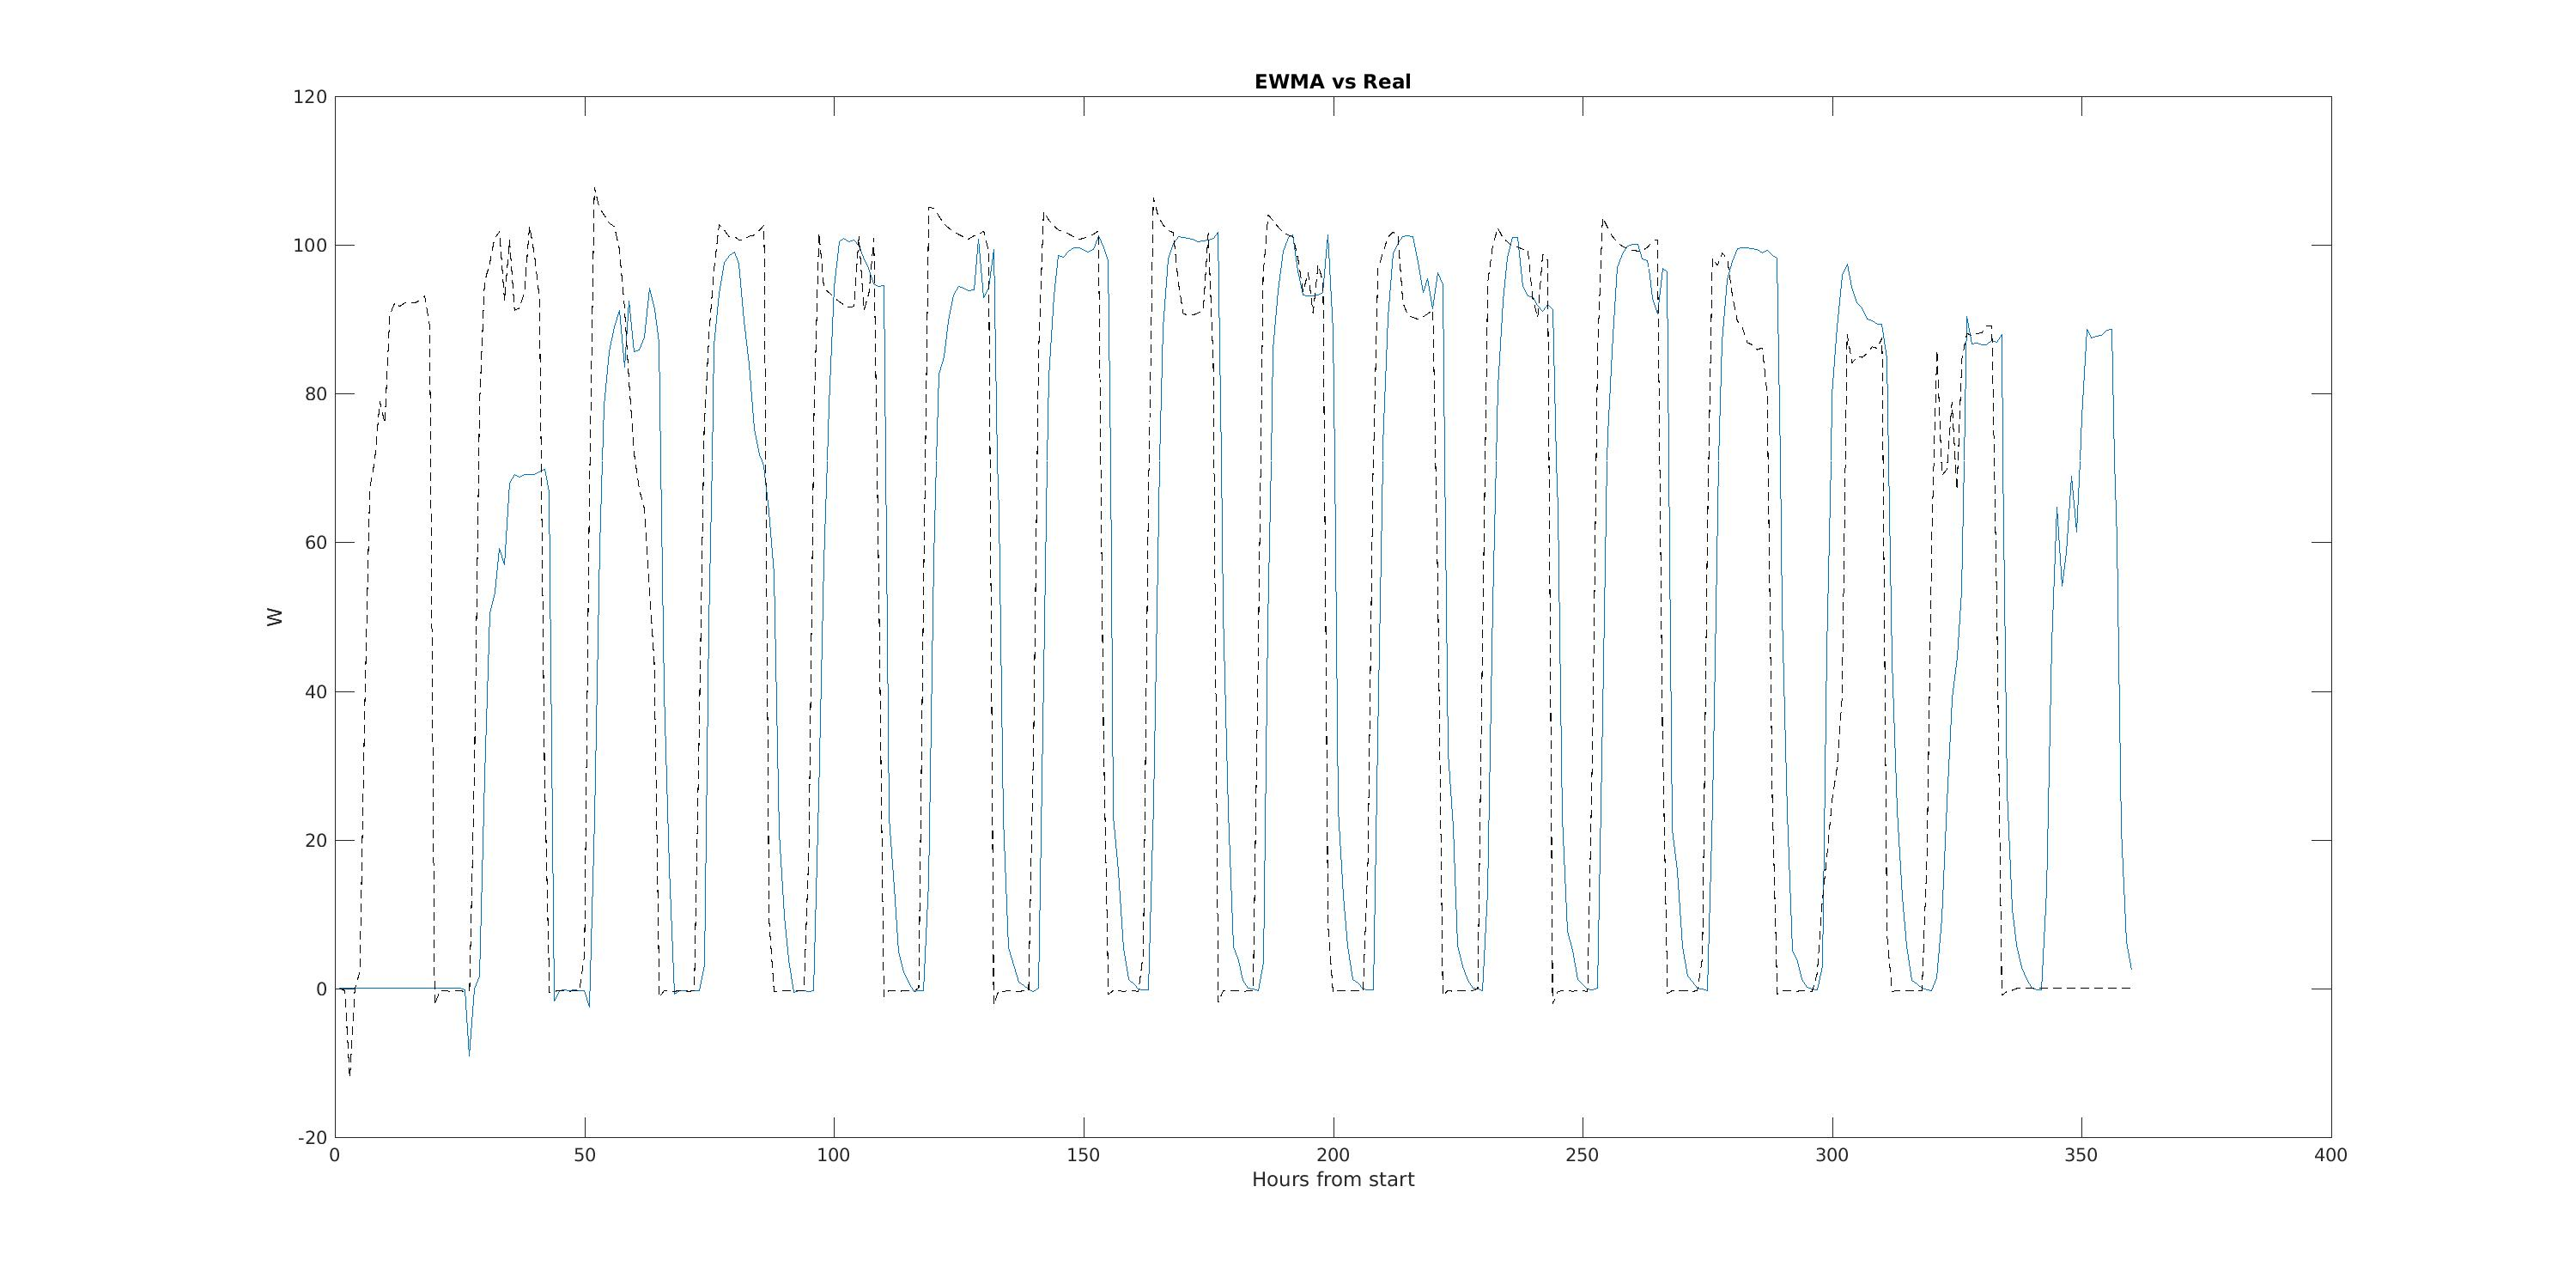
\includegraphics[width=\textwidth]{EWMA.jpg}
    \caption{EWMA Prediction accurancy}
    \label{fig:ewma_comp}
\end{figure}

\begin{figure}[h]
    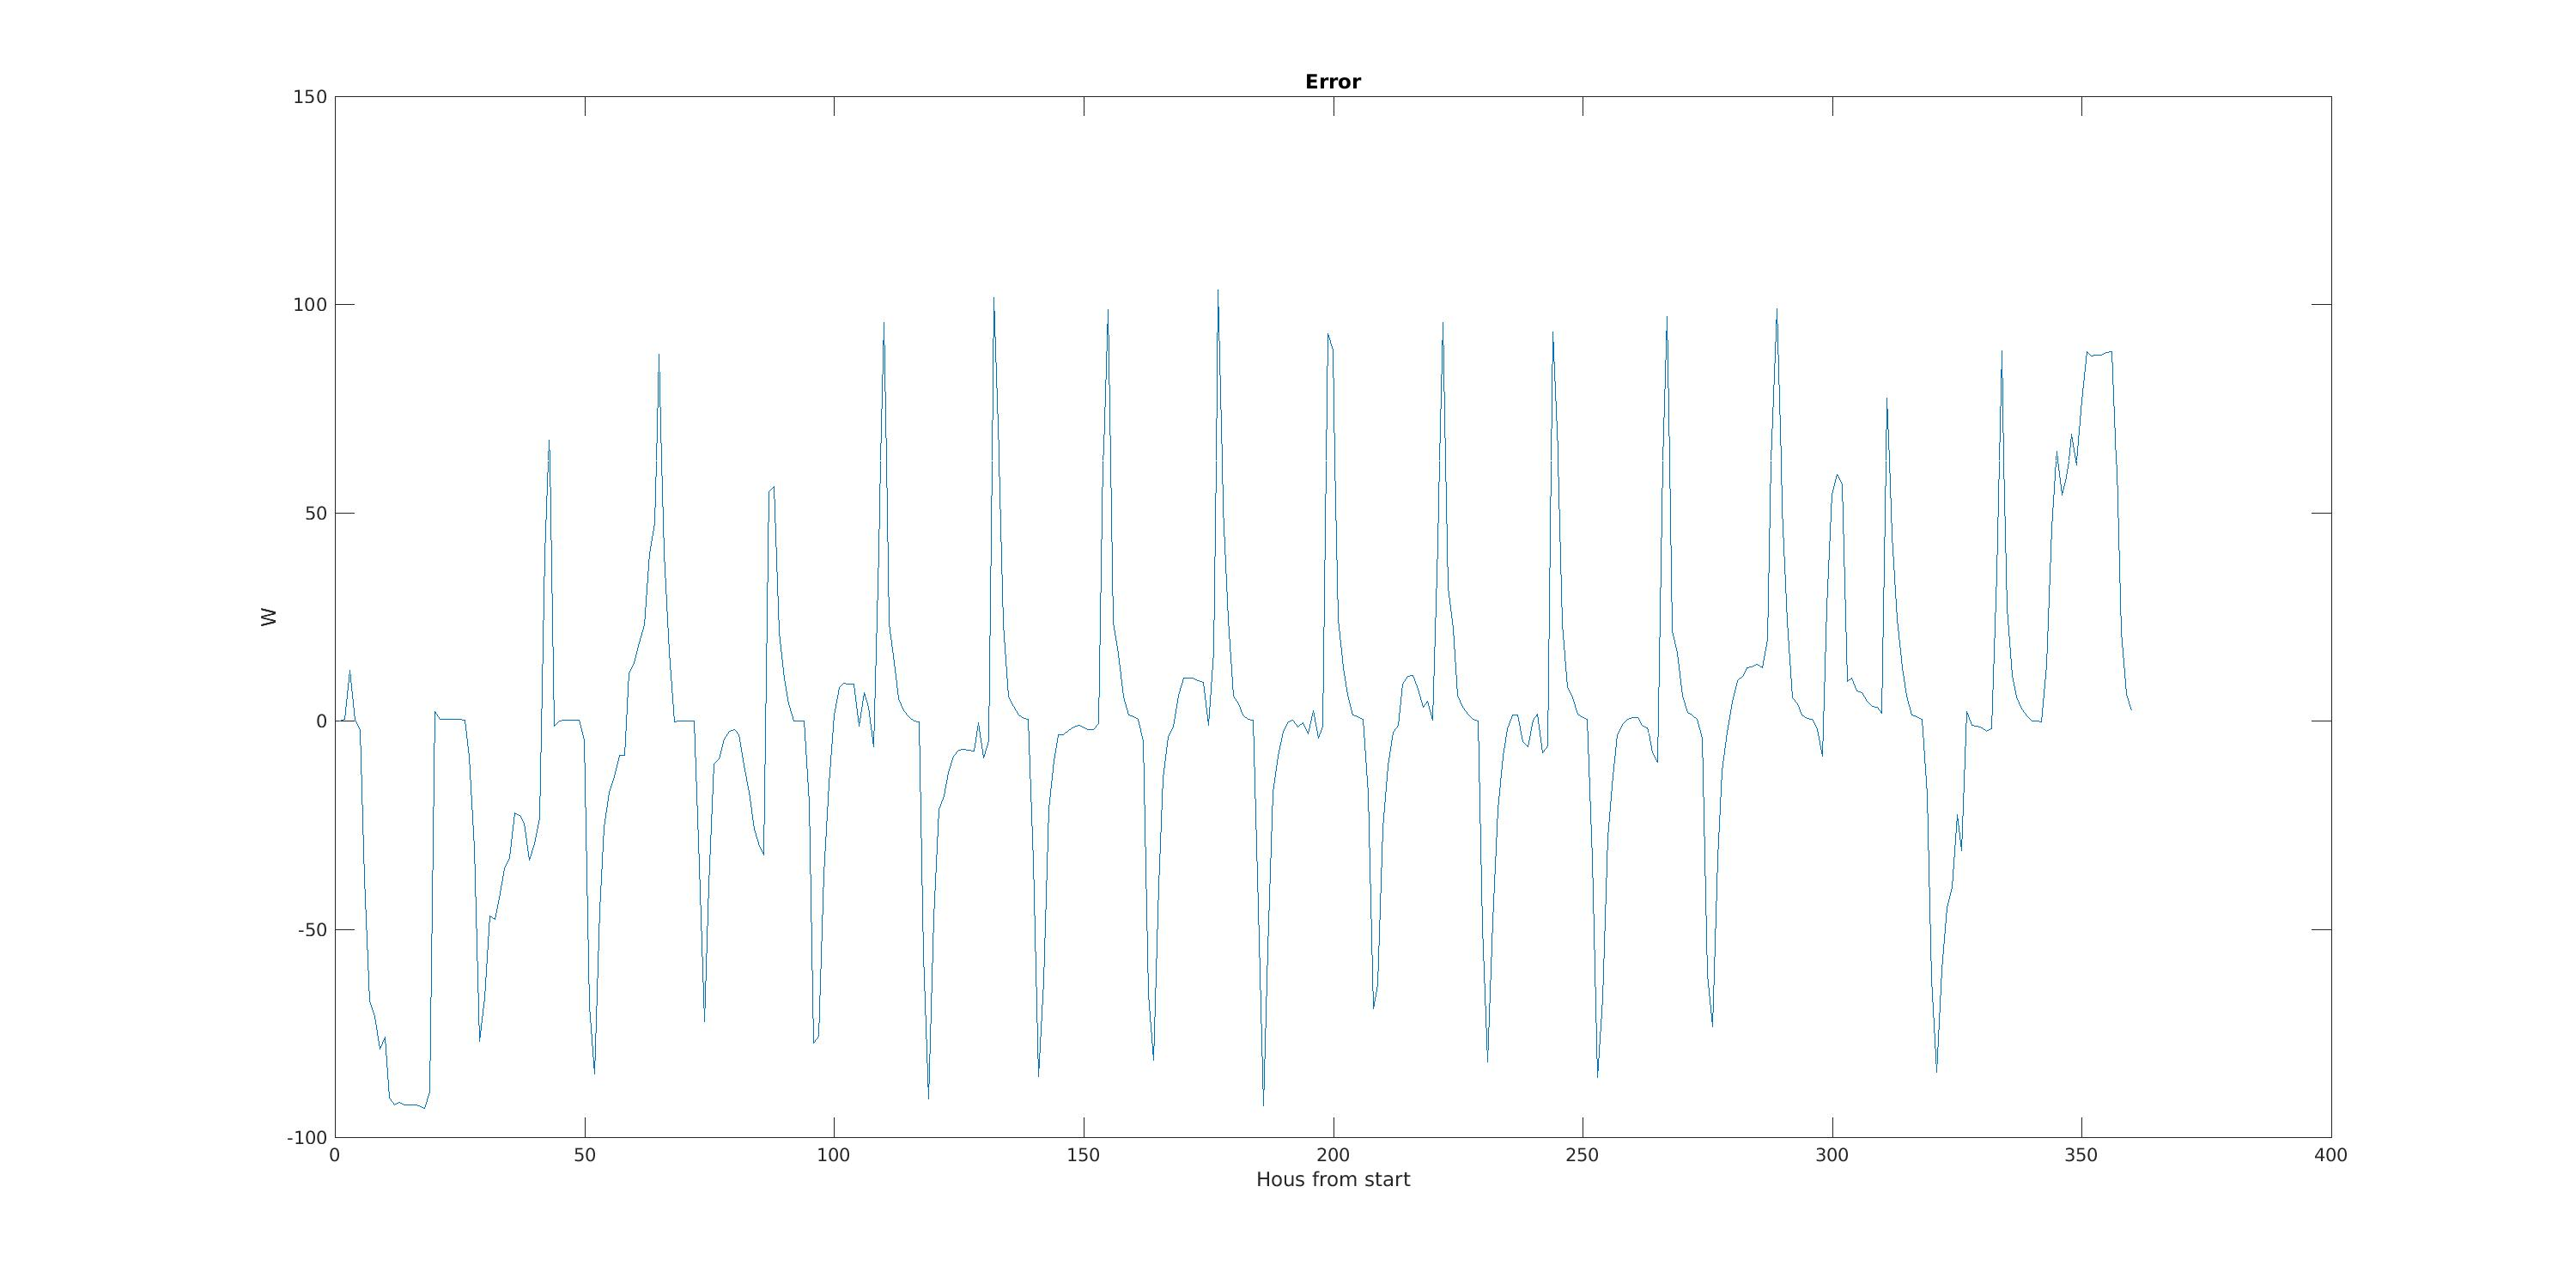
\includegraphics[width=\textwidth]{EWMA_error.jpg}
    \caption{EWMA Prediction error}
    \label{fig:ewma_error}
\end{figure}


\subsubsection{Adaptive power management (del ETHZ)}
 \label{ssub:adaptive_power_management}

El resultado de este tipo de predictor es muy similar al EWMA ya que realiza un cálculo basculado de el valor del dia anterior, pero sutilmente mejorado ya que tambien añade a la predicción los valores inmediatamente anteriores. El error en este caso es mas pronunciado en los extremos del dia pero mas estable en los puntos de irradiación estable.

Horizonte de predicción: 24h
$\alpha = TODO$

\begin{figure}[h]
    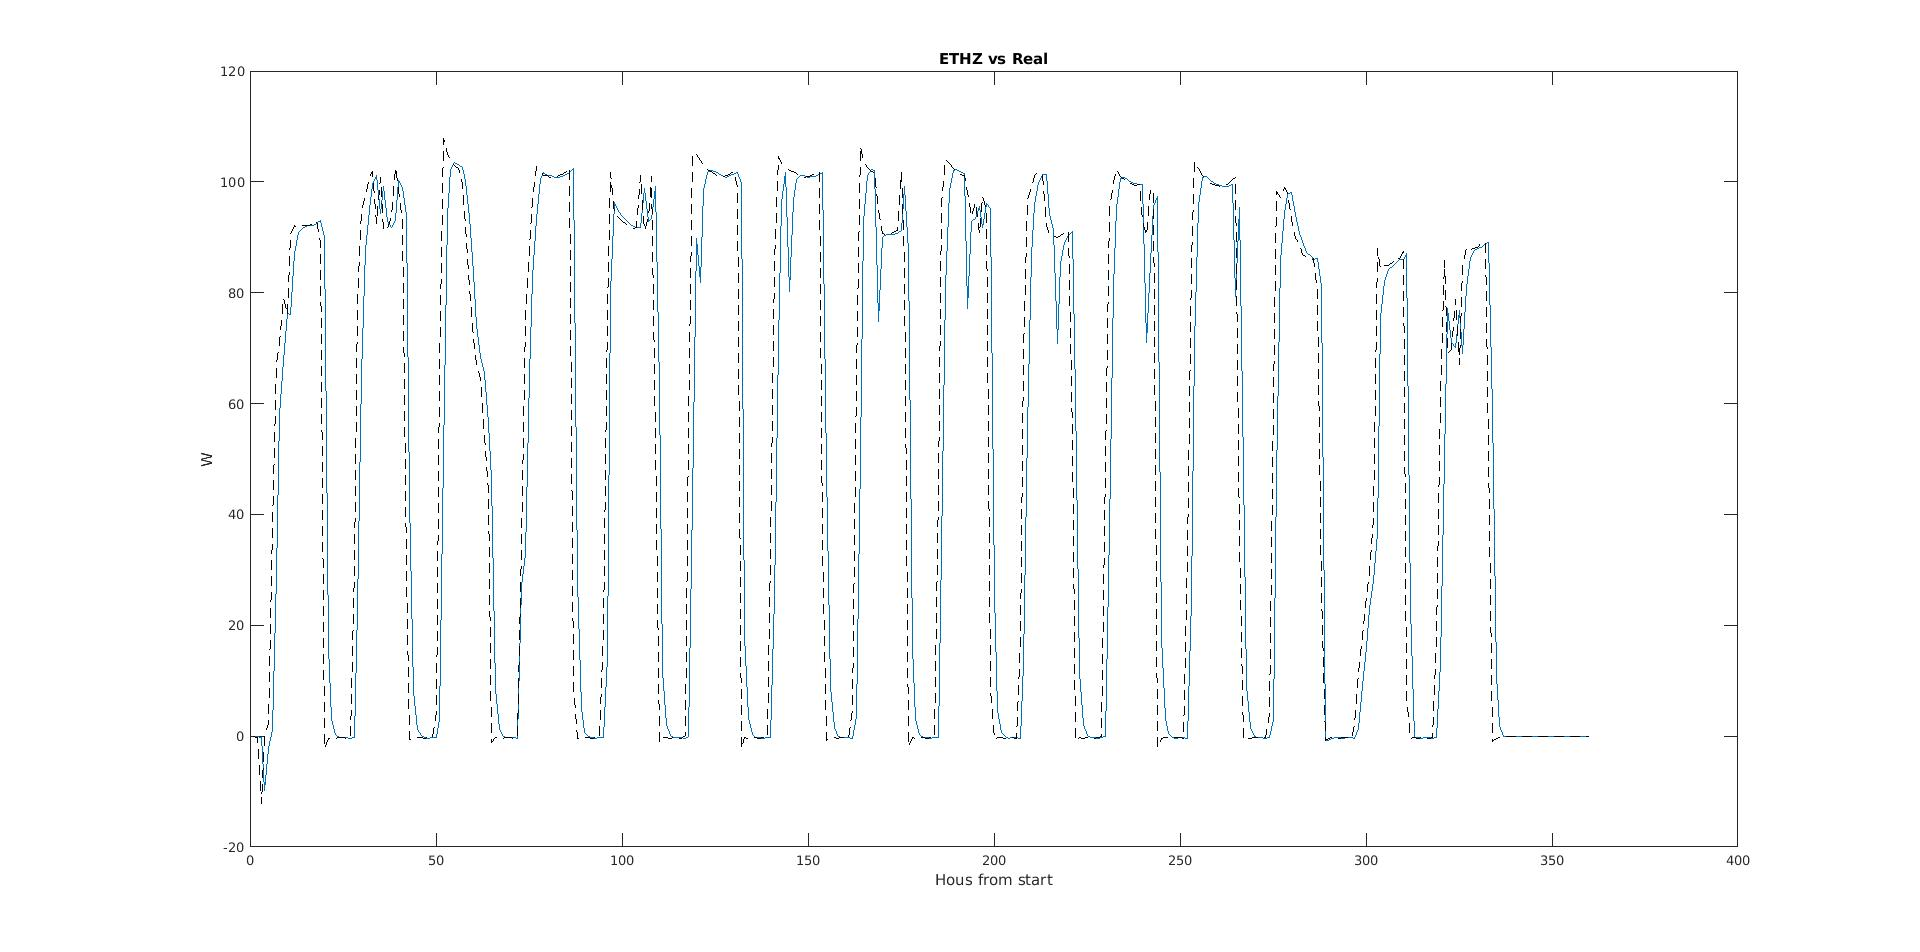
\includegraphics[width=\textwidth]{ETHZ.jpg}
    \caption{ETHZ Prediction accurancy}
    \label{fig:ethz_comp}
\end{figure}

\begin{figure}[h]
    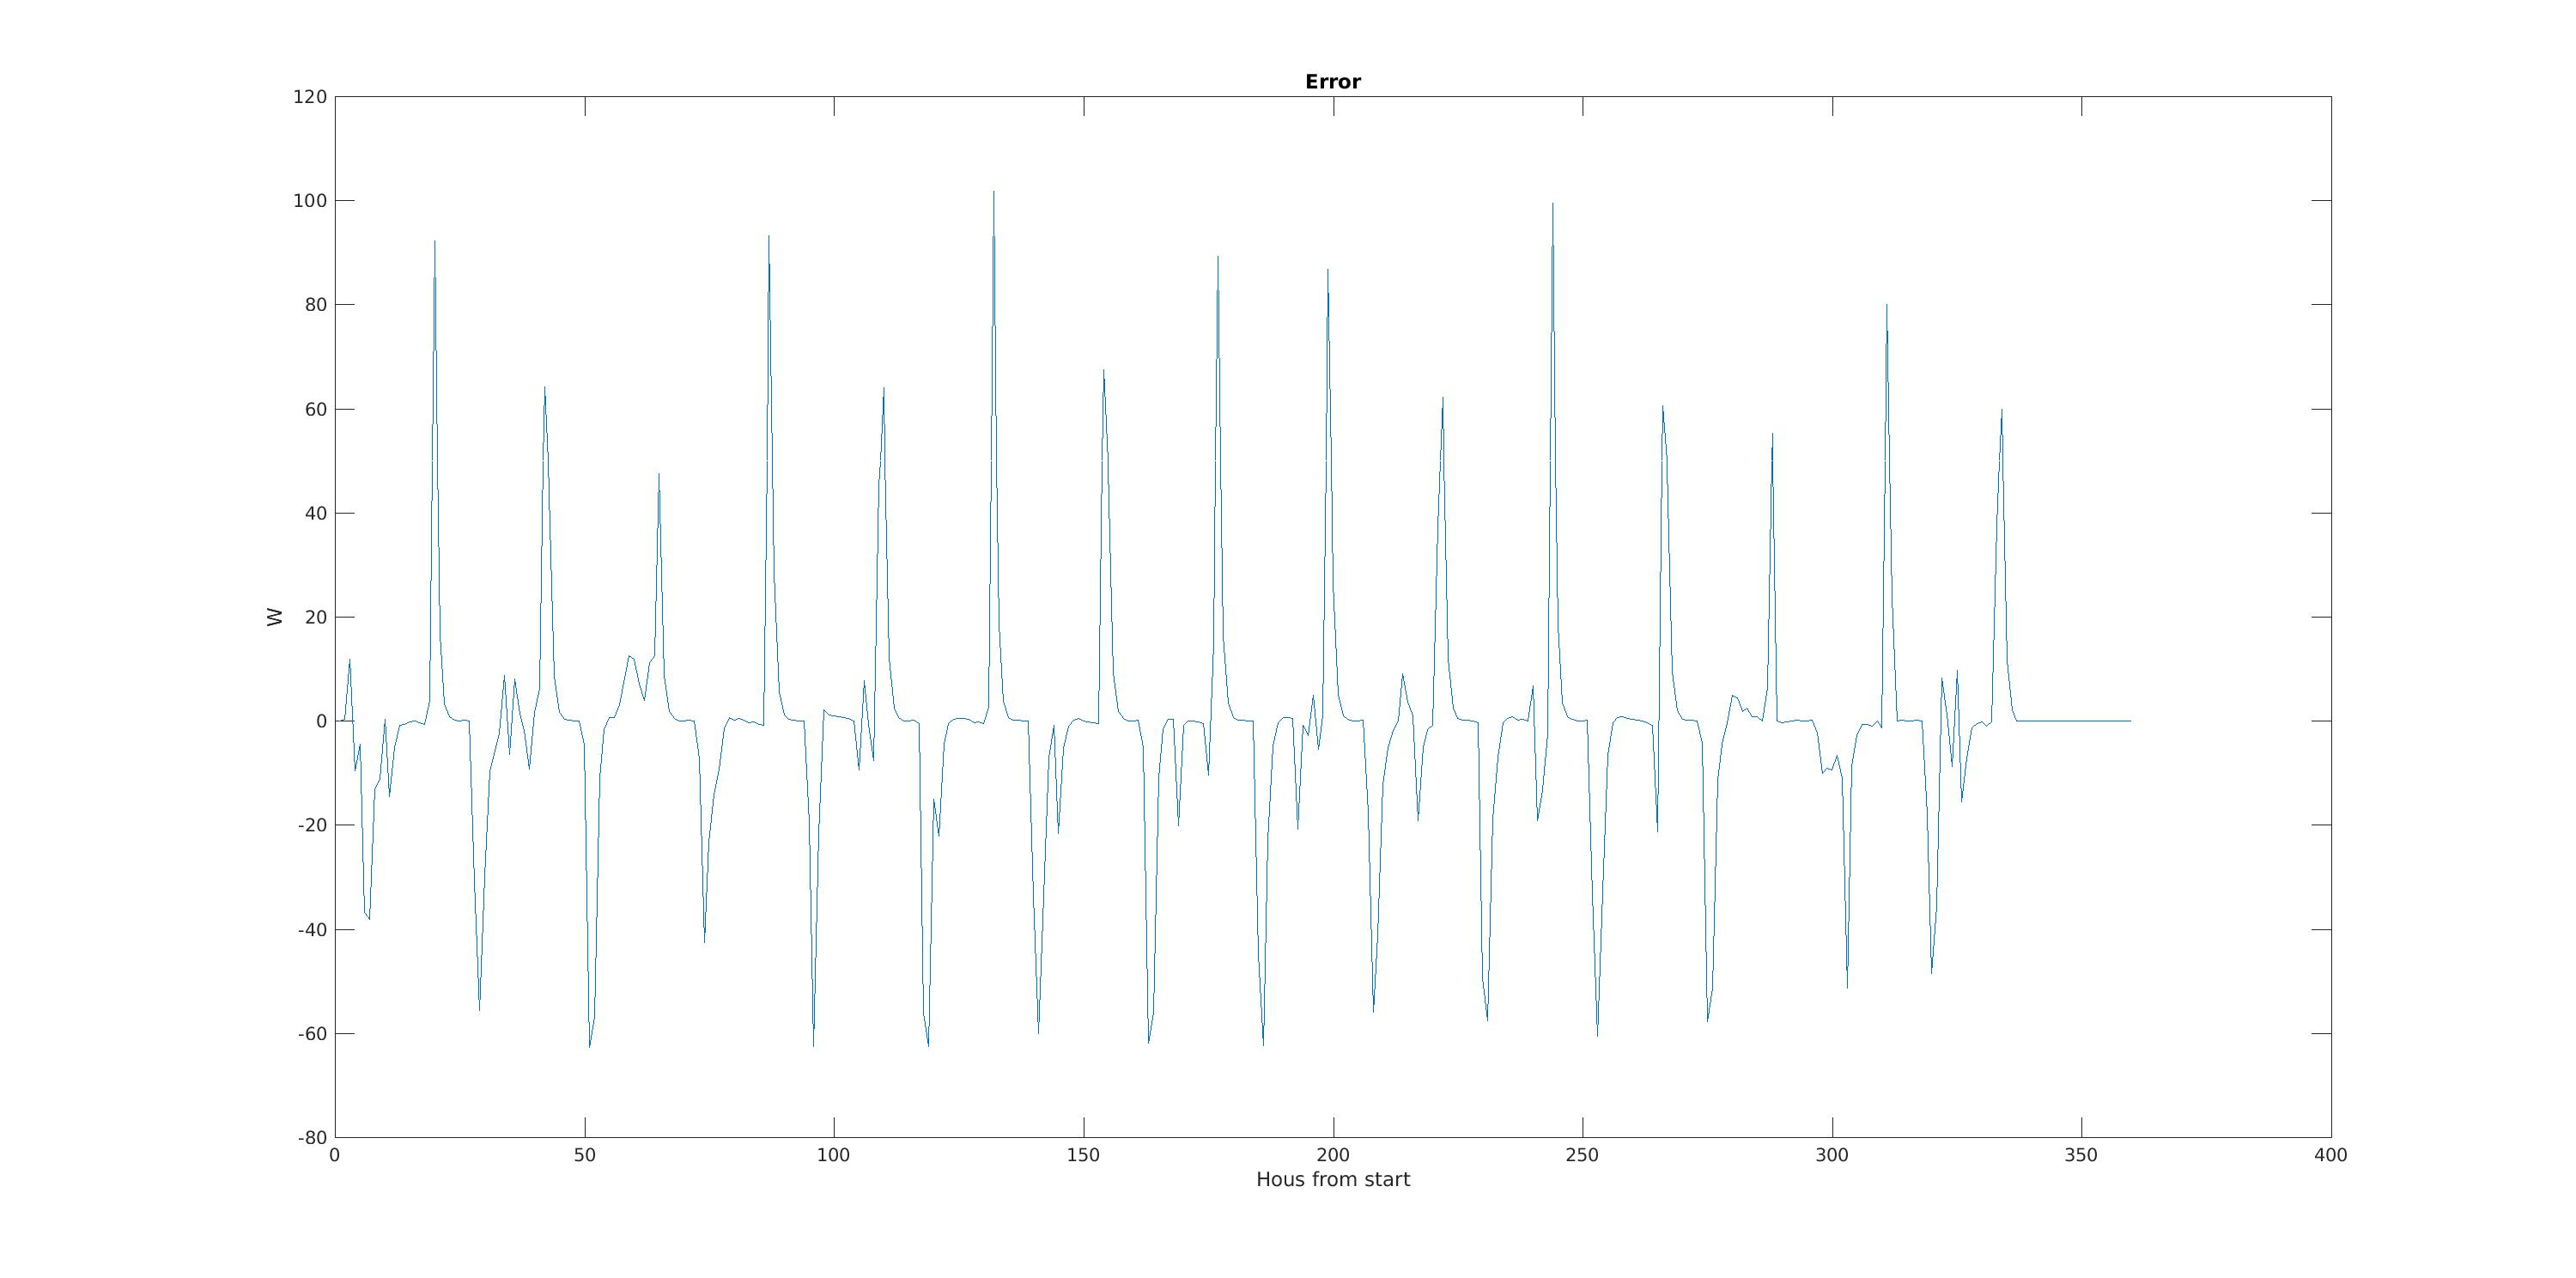
\includegraphics[width=\textwidth]{ETHZ_error.jpg}
    \caption{ETHZ Prediction error}
    \label{fig:ethz_error}
\end{figure}


\subsubsection{Optimal 2D prediction filter} 
\label{ssub:optimal_2d_prediction_filter}

\begin{figure}[h]
    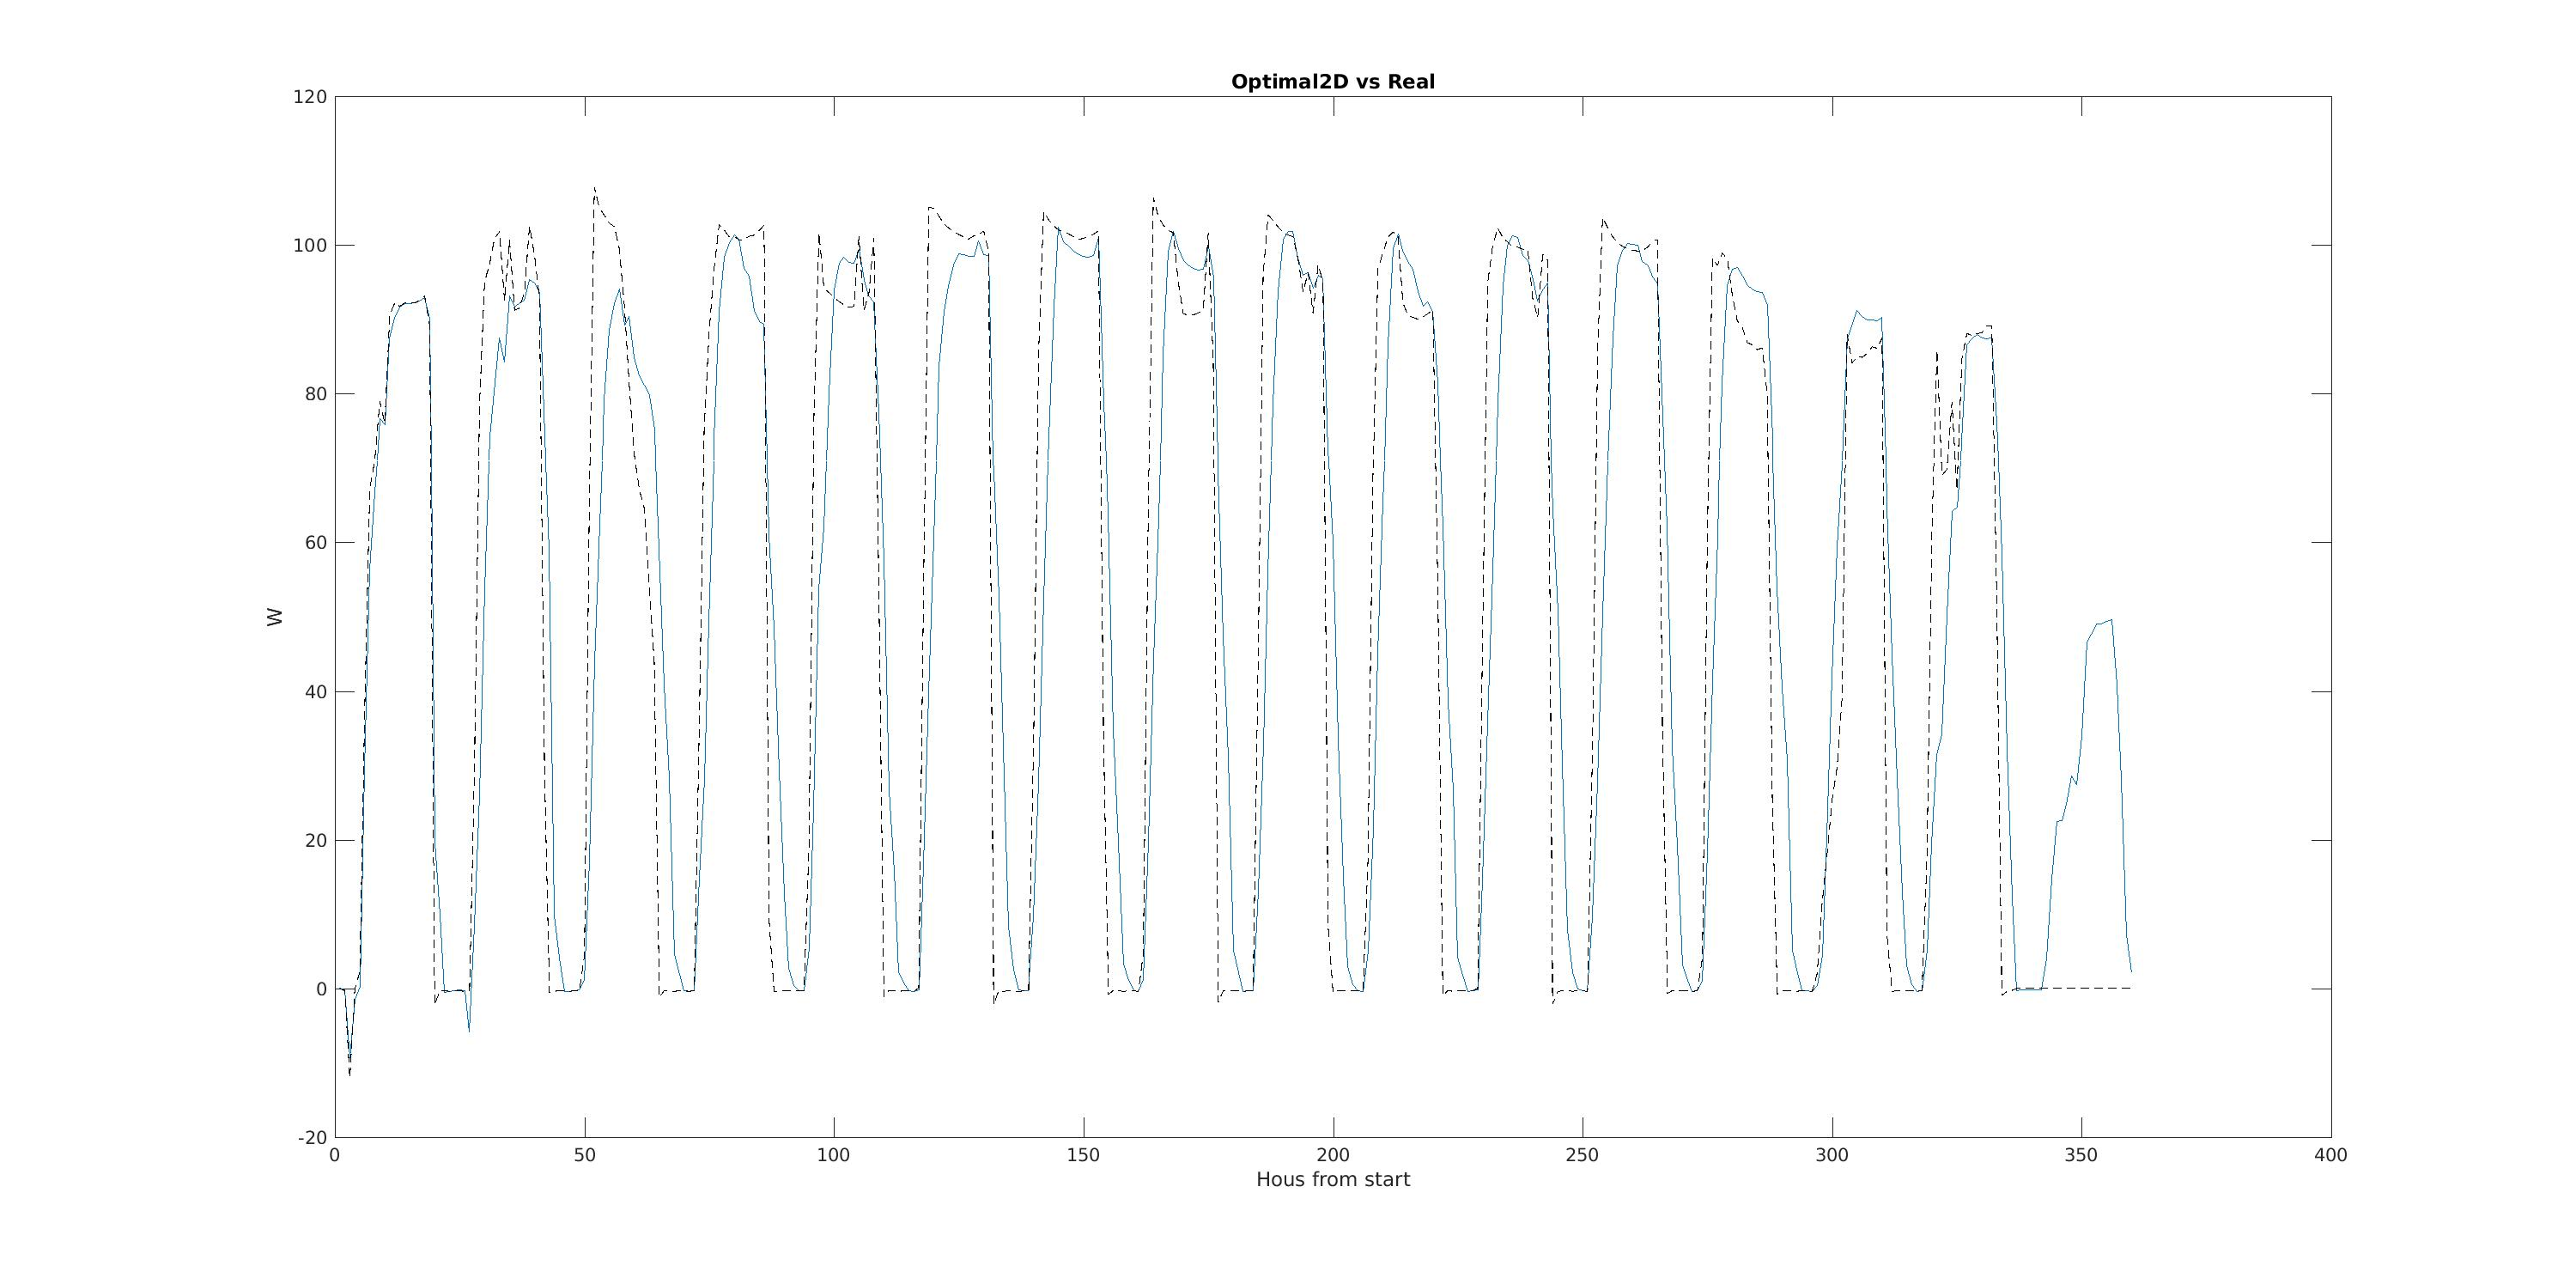
\includegraphics[width=\textwidth]{Optimal2D.jpg}
    \caption{2D filter Prediction accurancy}
    \label{fig:o2d_comp}
\end{figure}

\begin{figure}[h]
    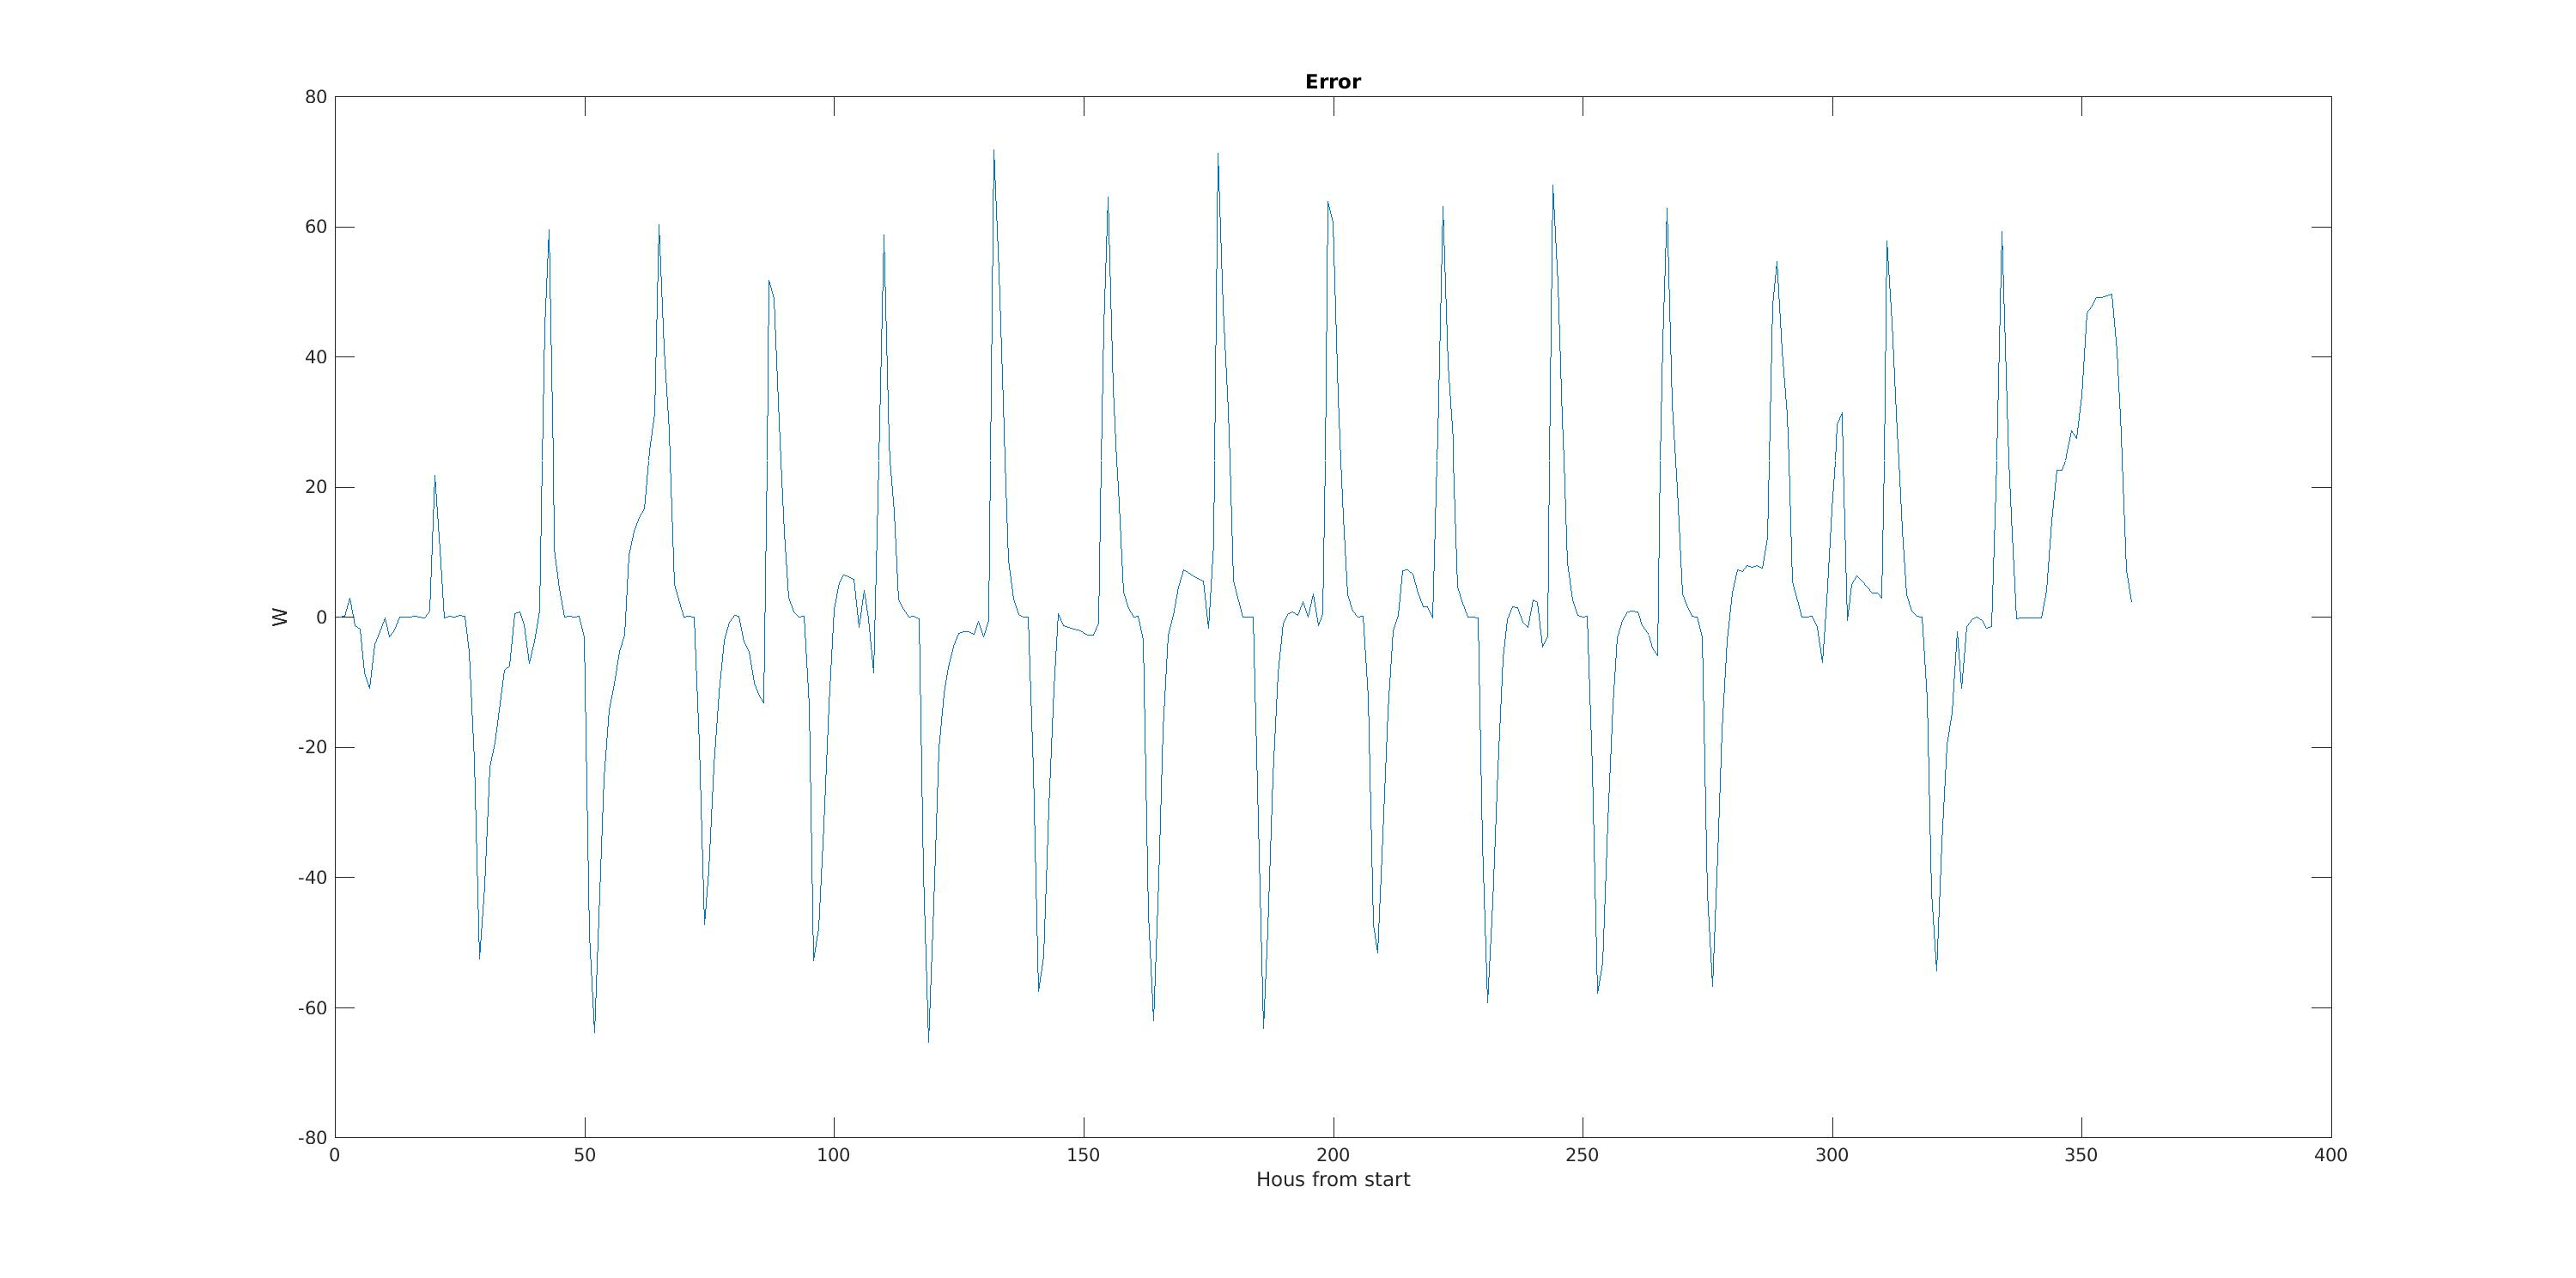
\includegraphics[width=\textwidth]{Optimal2D_error.jpg}
    \caption{2D filter Prediction error}
    \label{fig:o2d_error}
\end{figure}


\subsubsection{WCMA} 
\label{ssub:wcma}

\begin{figure}[h]
    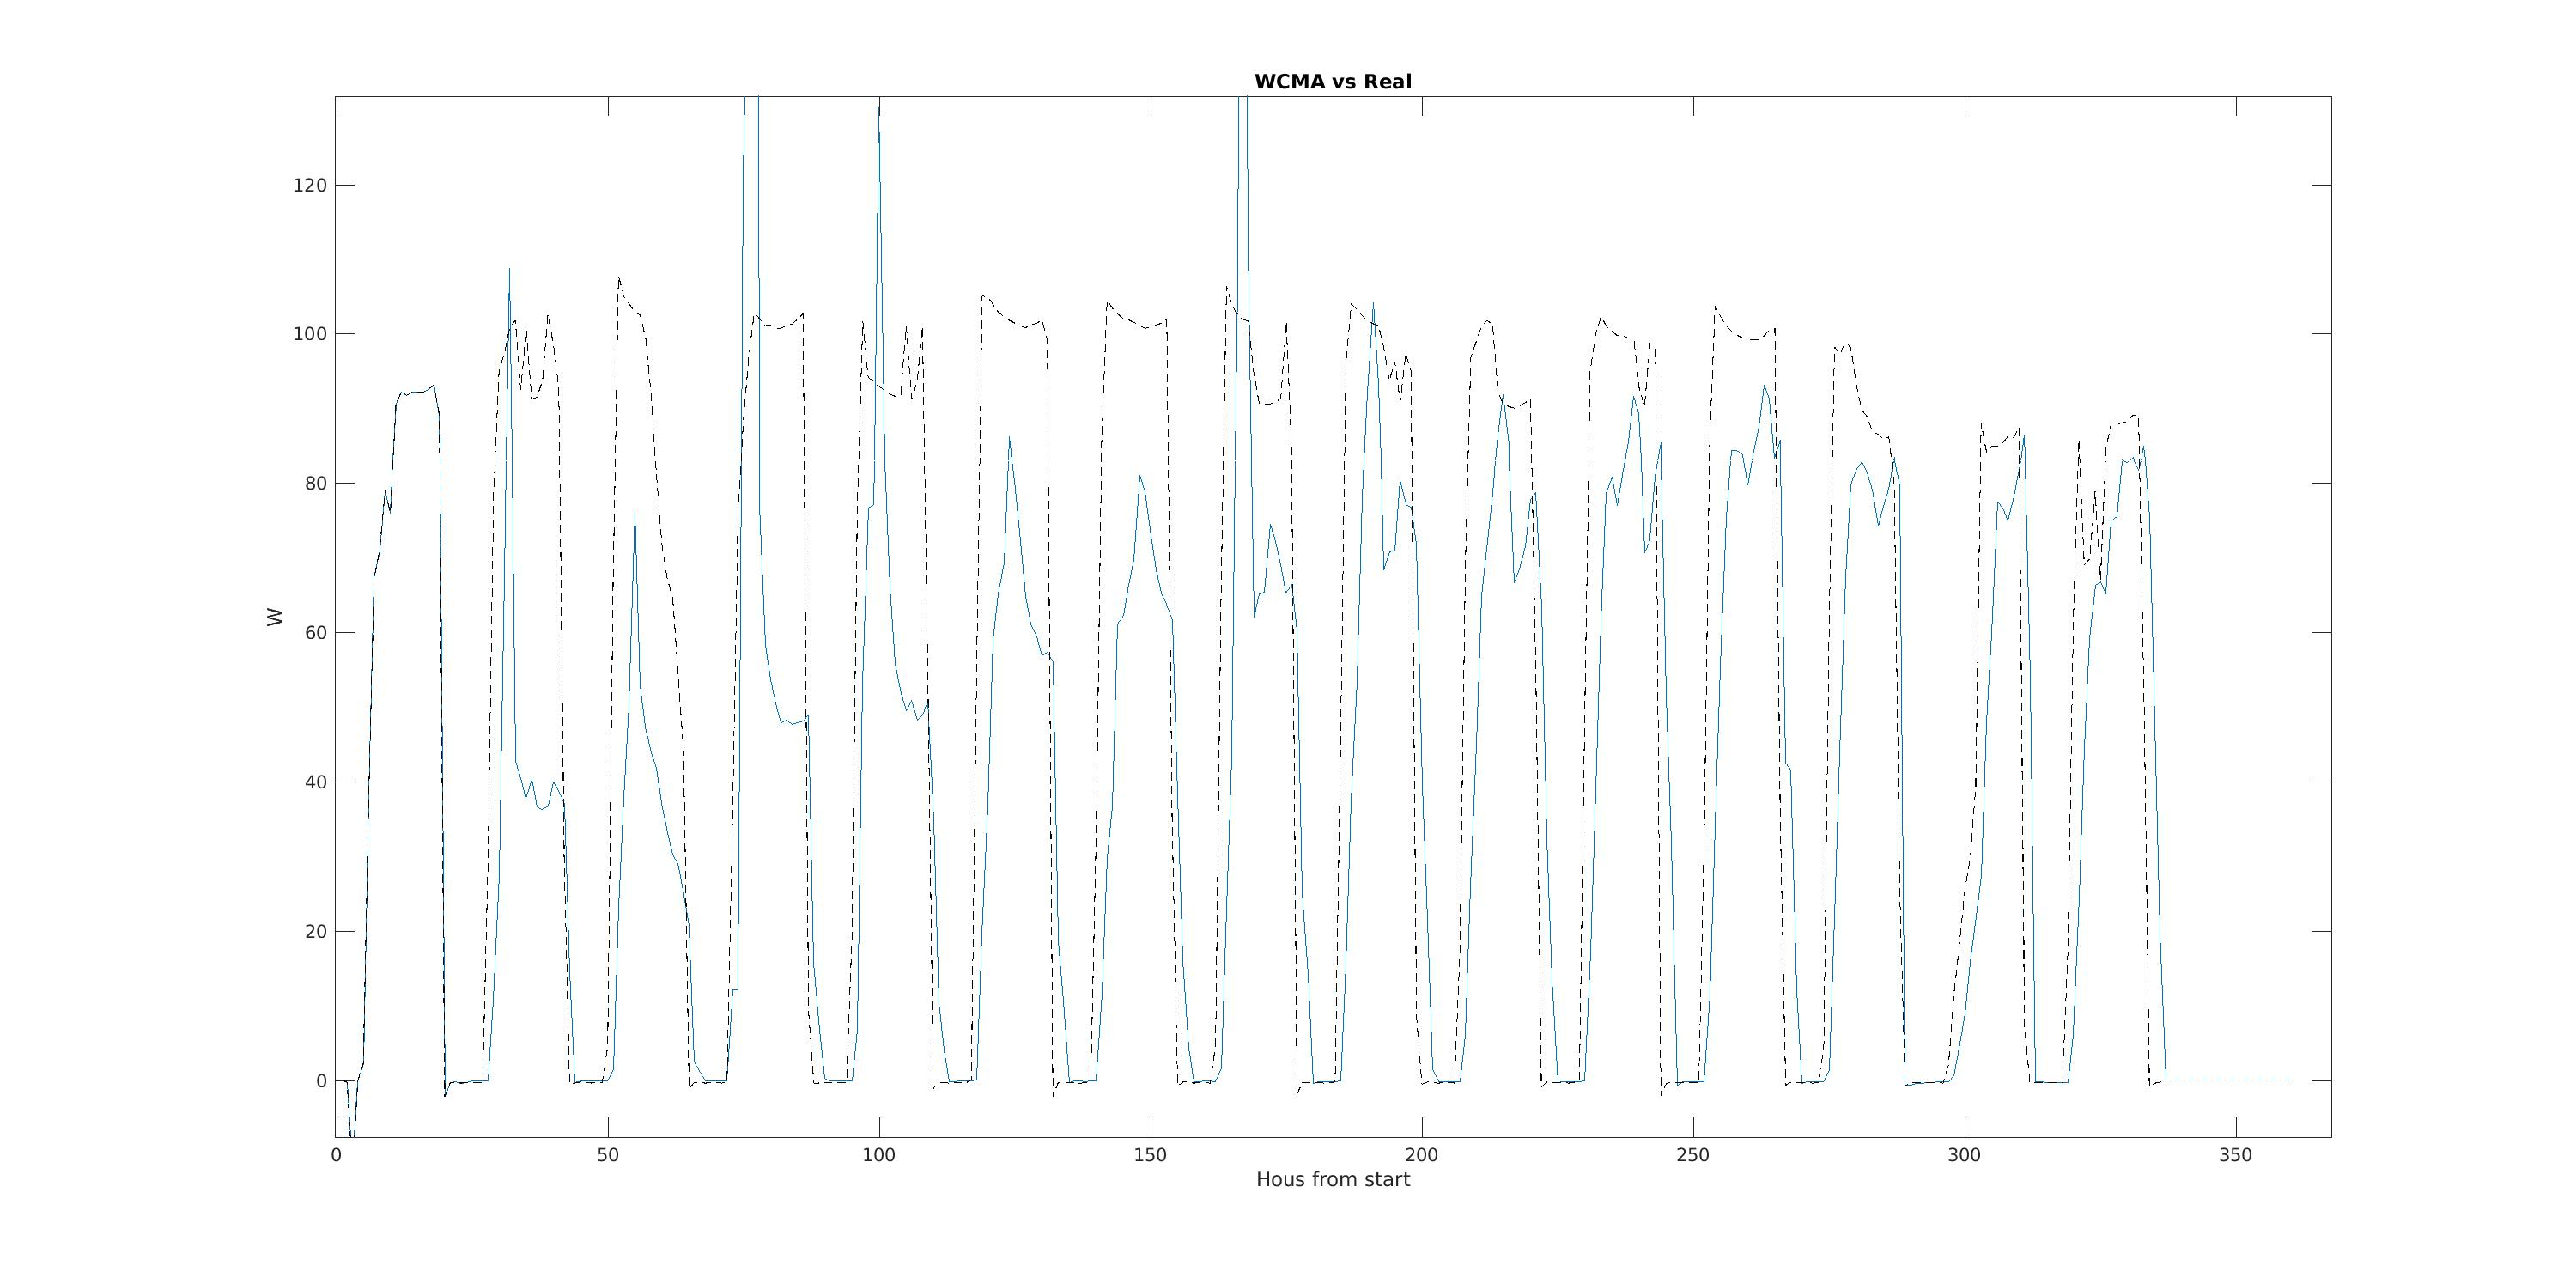
\includegraphics[width=\textwidth]{WCMA.jpg}
    \caption{WCMA Prediction accurancy}
    \label{fig:wcma_comp}
\end{figure}

\begin{figure}[h]
    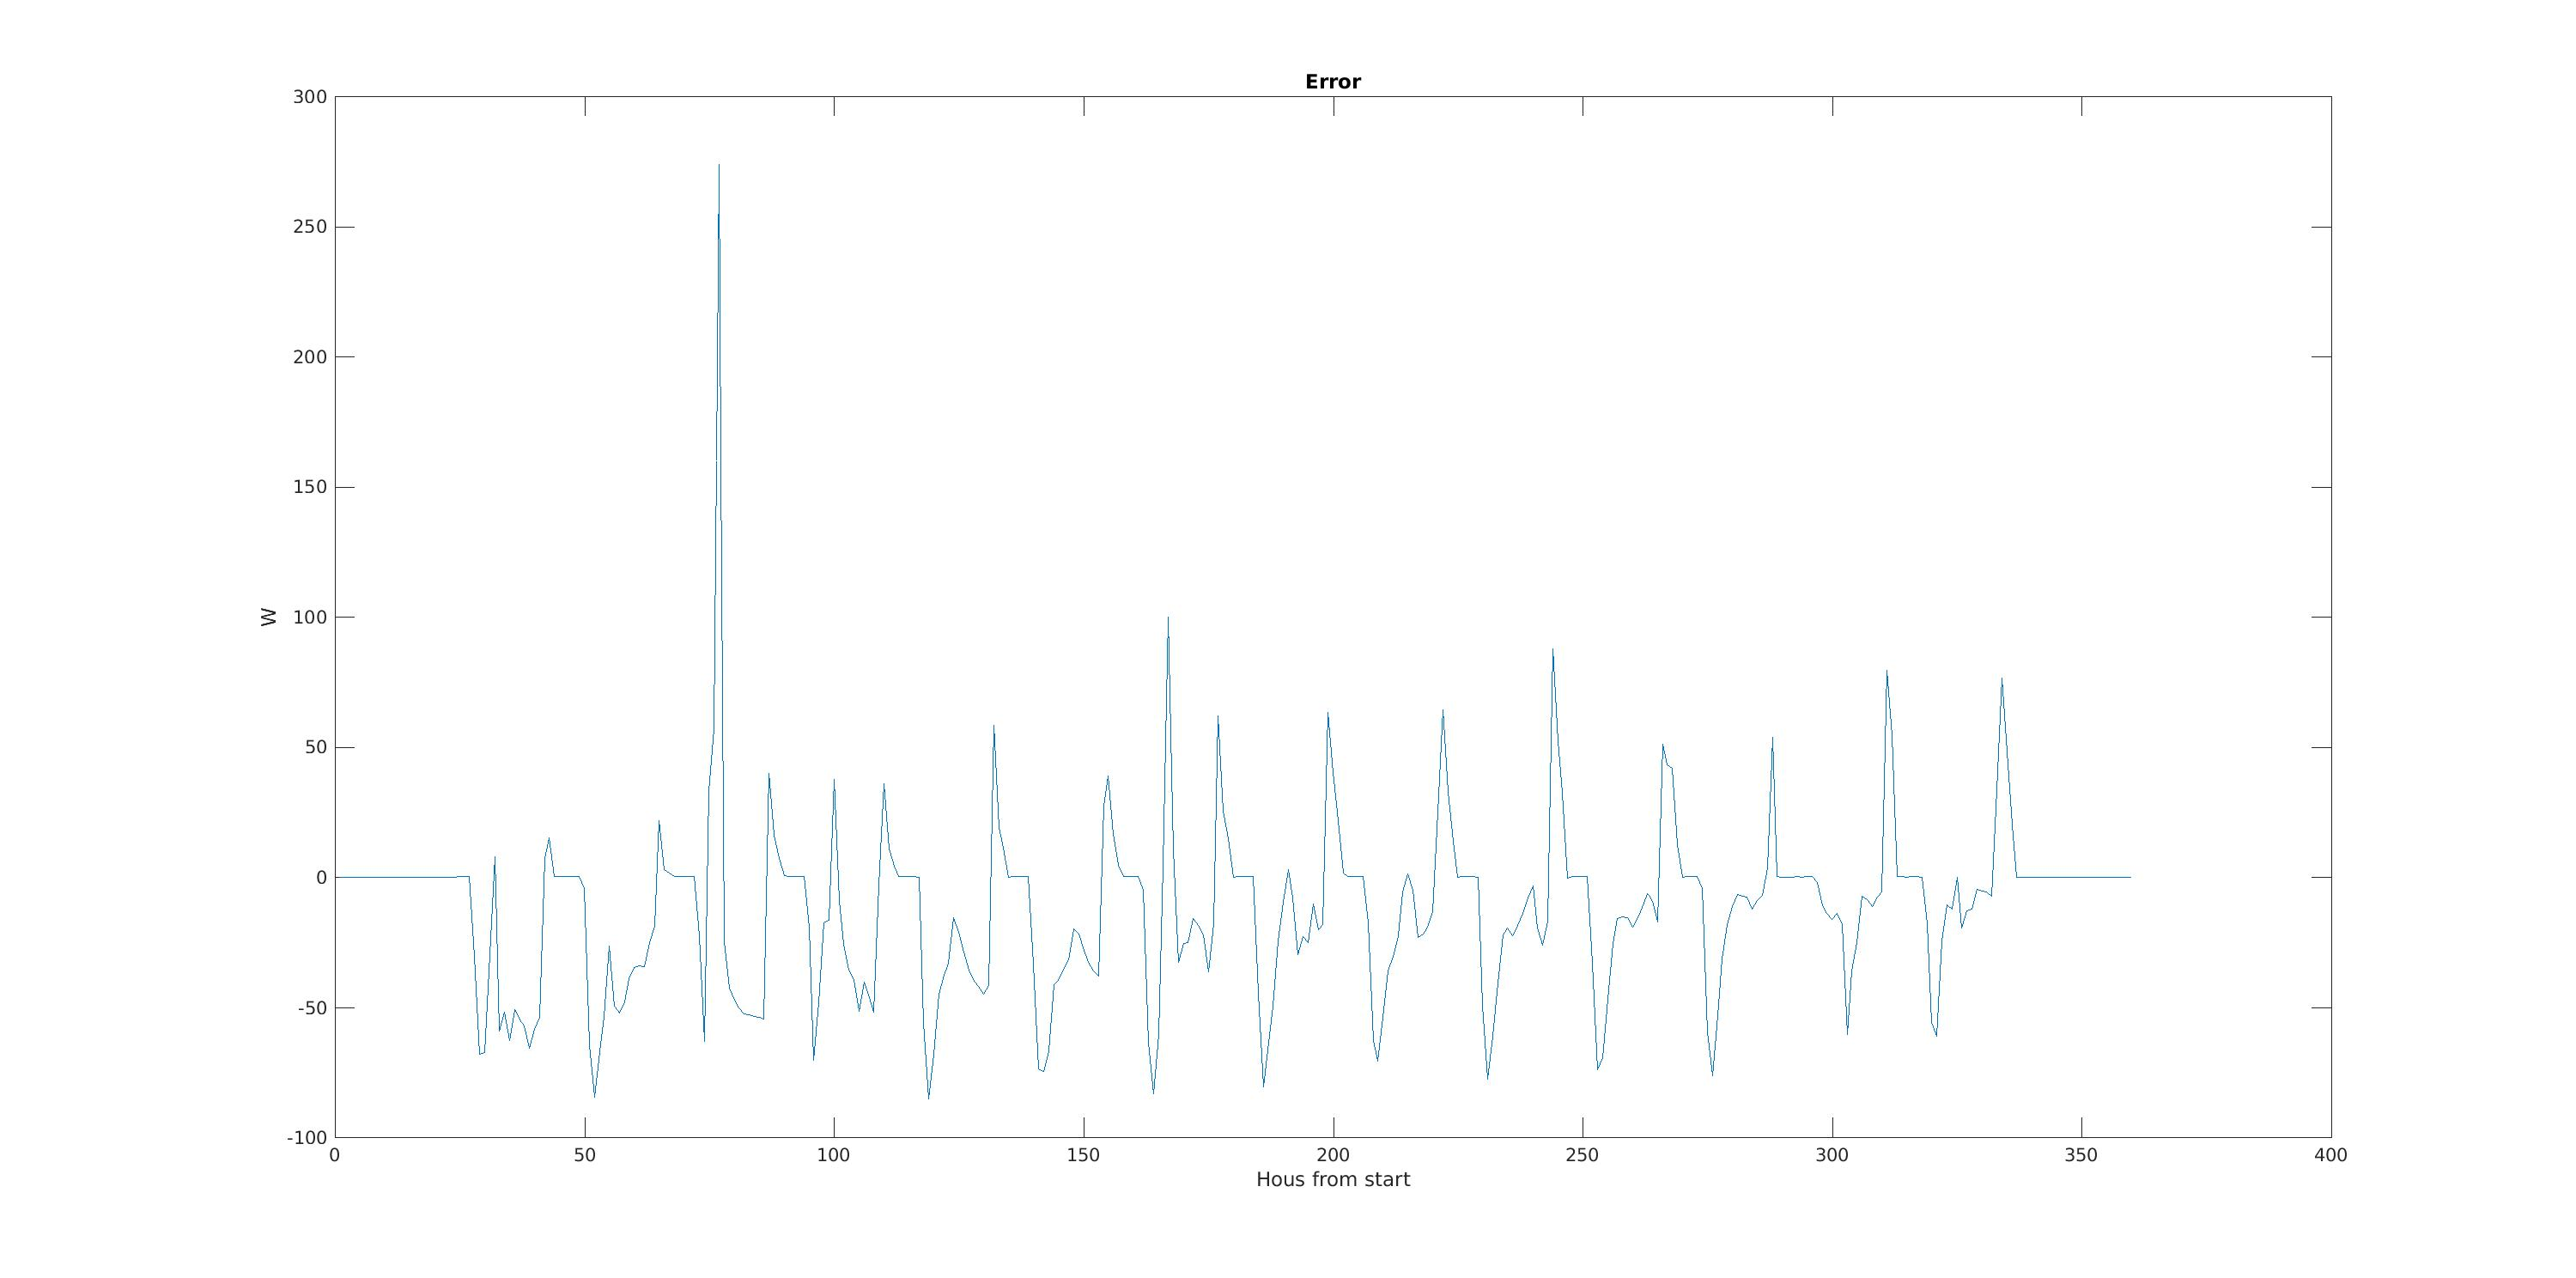
\includegraphics[width=\textwidth]{WCMA_error.jpg}
    \caption{WCMA Prediction error}
    \label{fig:wcma_error}
\end{figure}


\subsubsection{WCMA with PDR} 
\label{ssub:wcma_with_pdr}

\begin{figure}[h]
    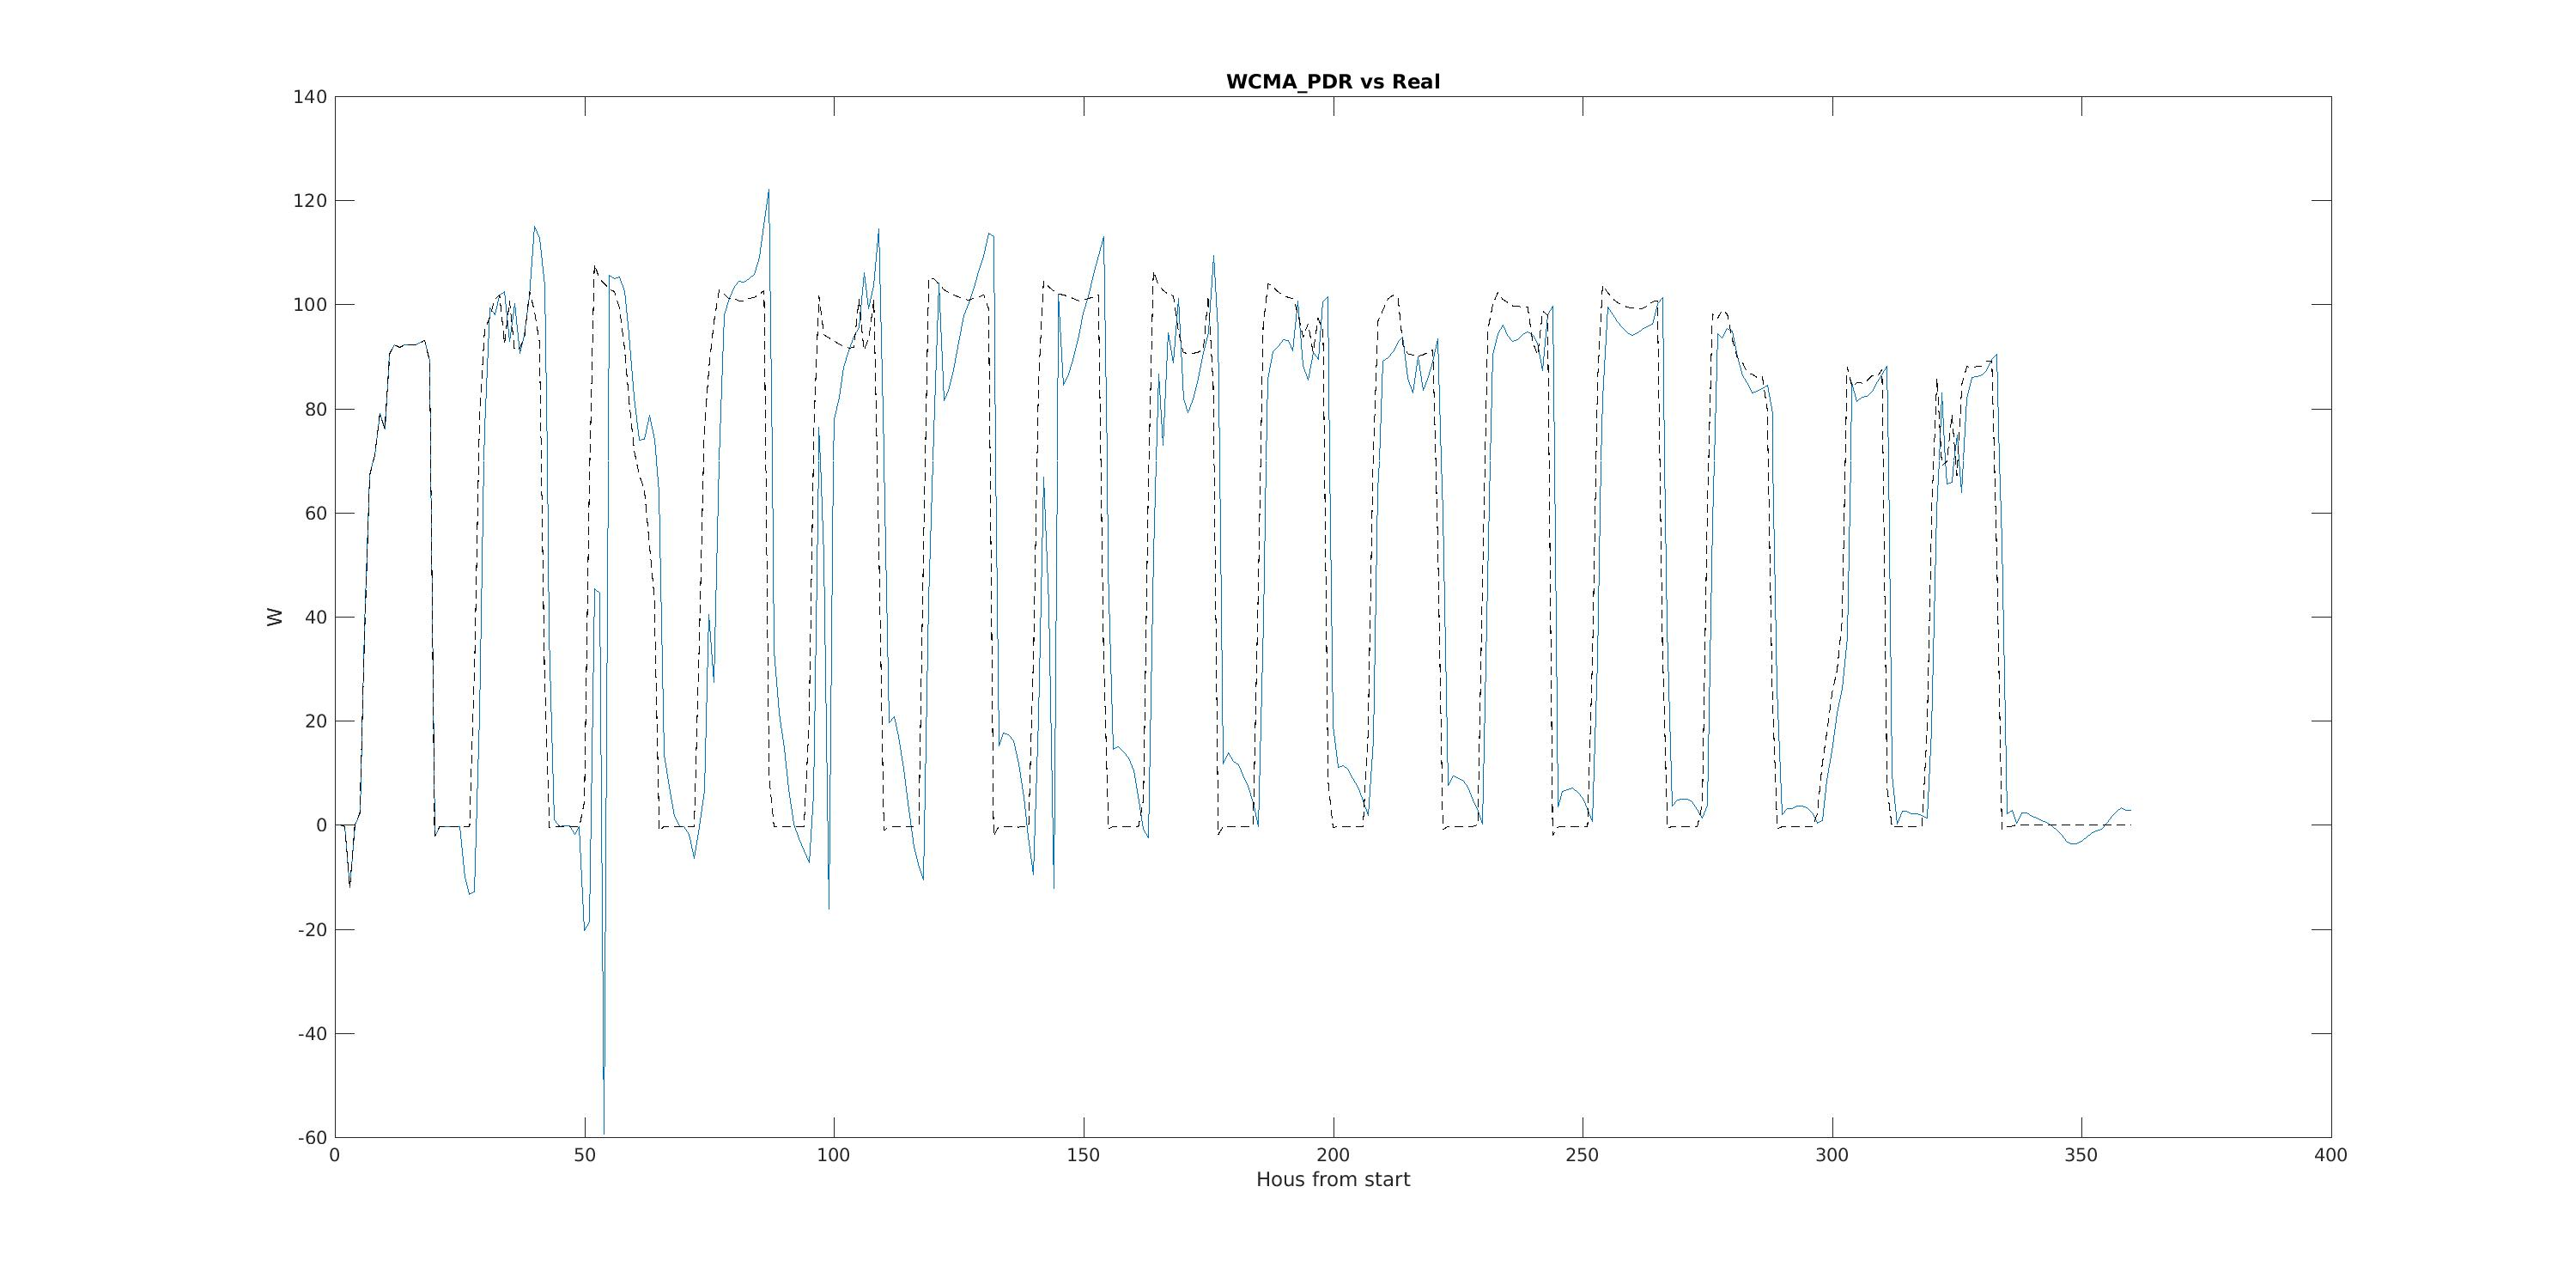
\includegraphics[width=\textwidth]{WCMA-PDR.jpg}
    \caption{WCMA with PDR Prediction accurancy}
    \label{fig:wcmapdr_comp}
\end{figure}

\begin{figure}[h]
    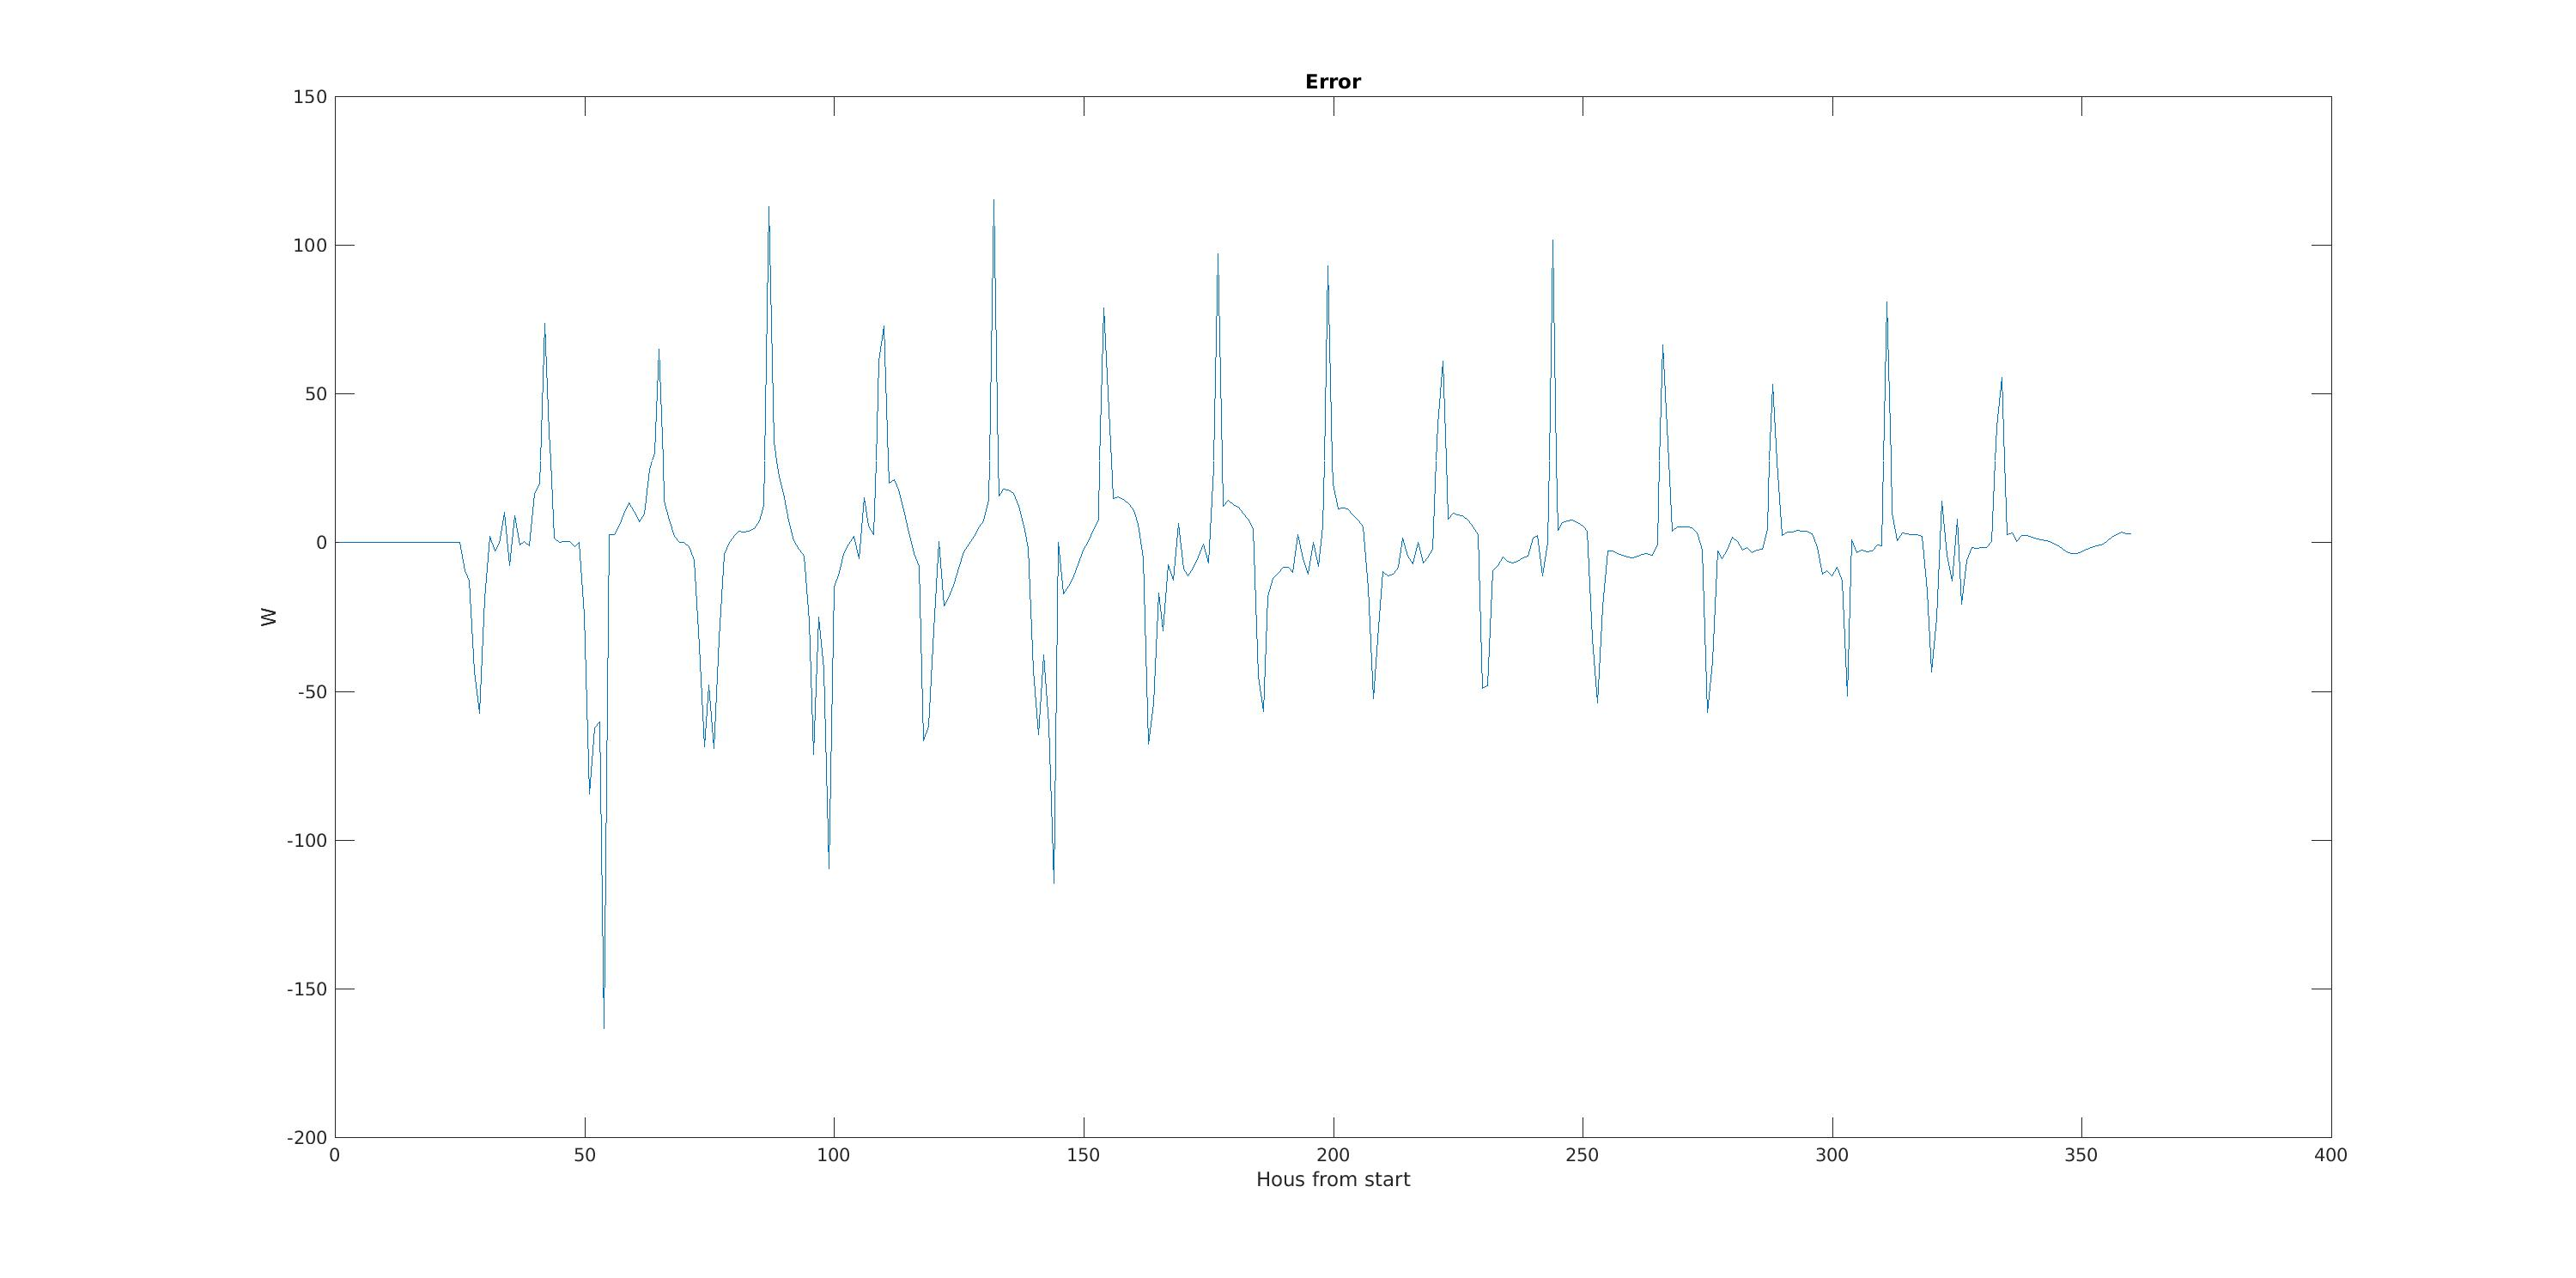
\includegraphics[width=\textwidth]{WCMA-PDR_error.jpg}
    \caption{WCMA with PDR Prediction error}
    \label{fig:wcmapdr_error}
\end{figure}


\subsubsection{Red neuronal artificial} 
\label{ssub:nn}

El resultado de la red neuronal es especialmente bueno si consideramos valores estables, pero el tiempo de procesado y aprendizaje (El cual deberá ser continuo)

\begin{figure}[h]
    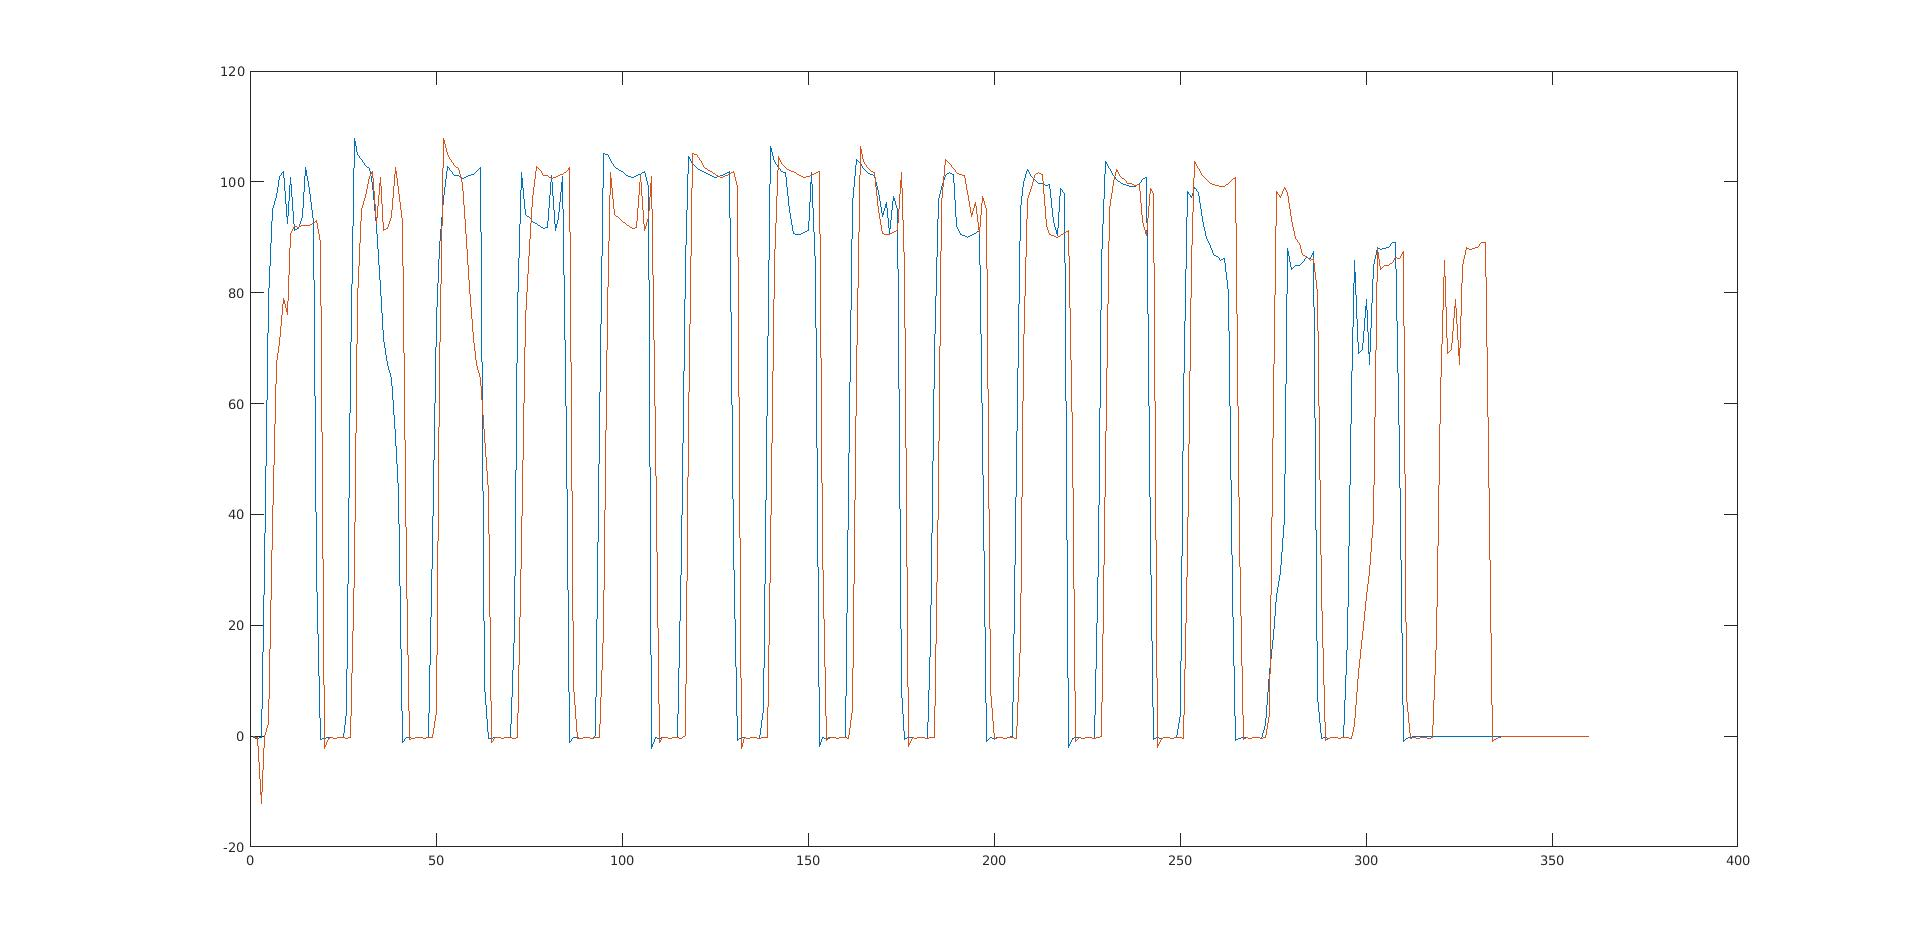
\includegraphics[width=\textwidth]{nn.jpg}
    \caption{neural network Prediction accurancy}
    \label{fig:nn_comp}
\end{figure}

\begin{figure}[h]
    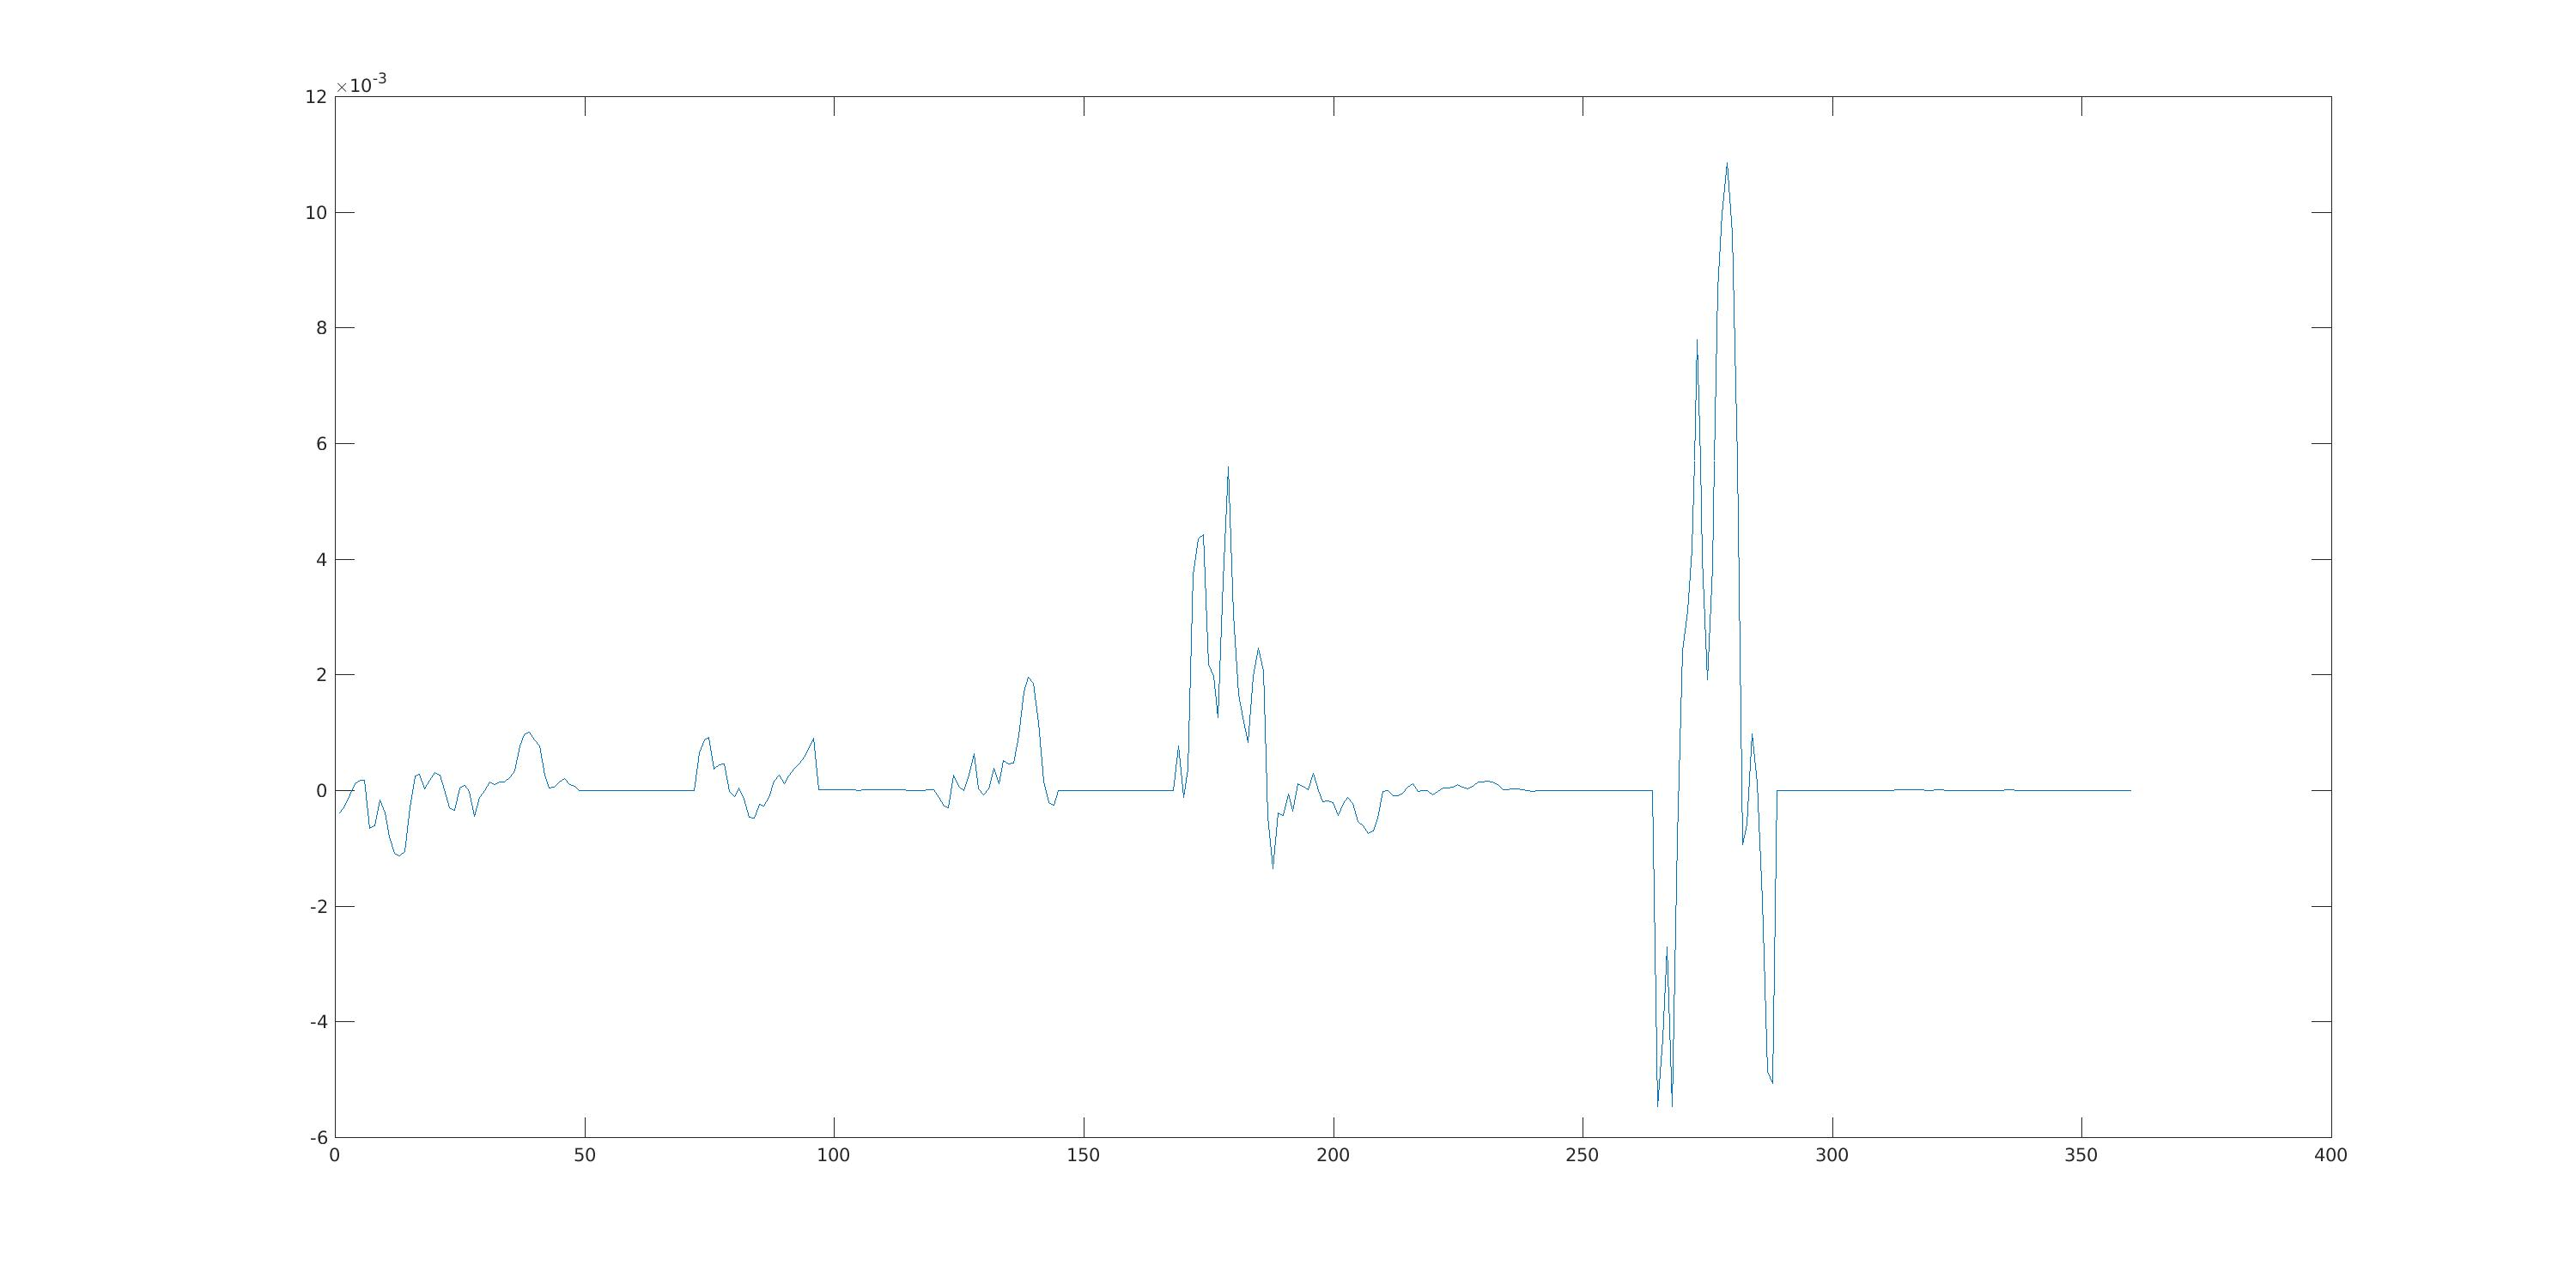
\includegraphics[width=\textwidth]{nn_error.jpg}
    \caption{neural network Prediction error}
    \label{fig:nn_error}
\end{figure}


\subsubsection{N4SID} 
\label{ssub:n4sid}

\begin{figure}[h]
    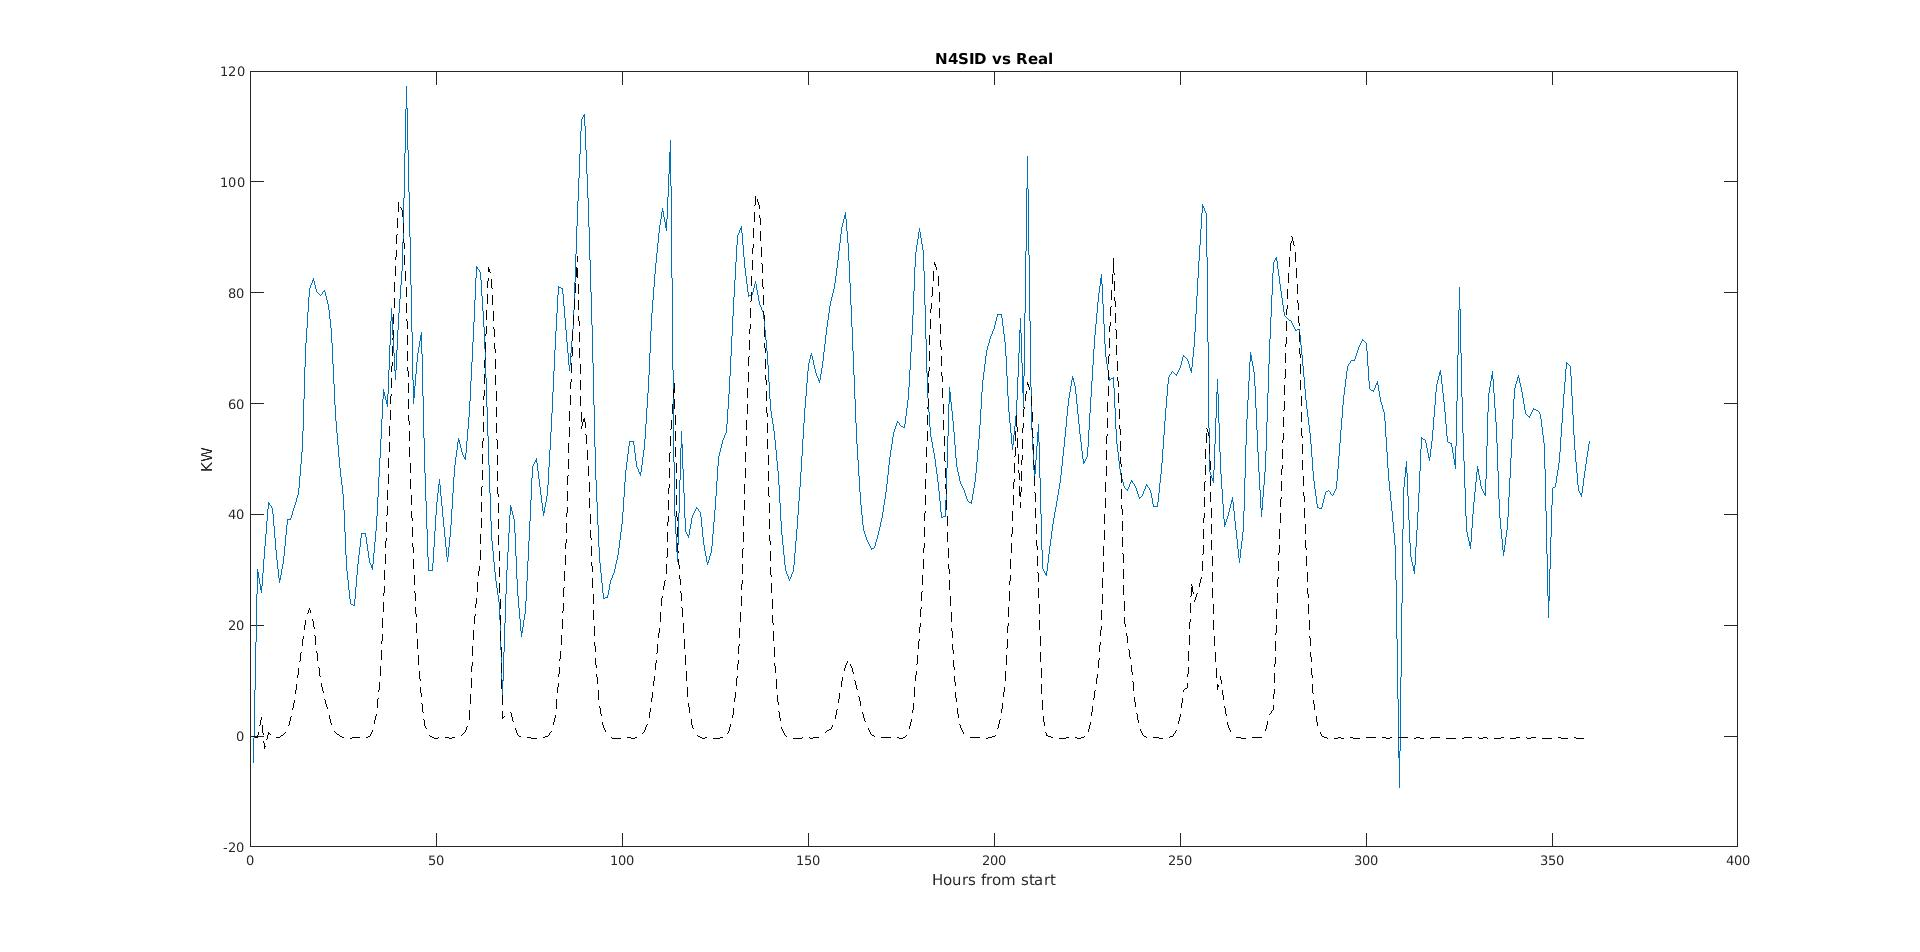
\includegraphics[width=\textwidth]{n4sid_solar.jpg}
    \caption{N4SID Prediction accurancy}
\end{figure}




\section{Eólica: Modelos}
\label{sub:Modelos}

Para el estudio de predicción de energía eólica se han probado los siguientes modelos.

\begin{itemize}
    \item N4SID
    \item ARIMA/ARMA
\end{itemize}

\subsubsection{Eólica: N4SID} % (fold)
\label{ssub:eólica_n4sid}


\begin{figure}[h]
    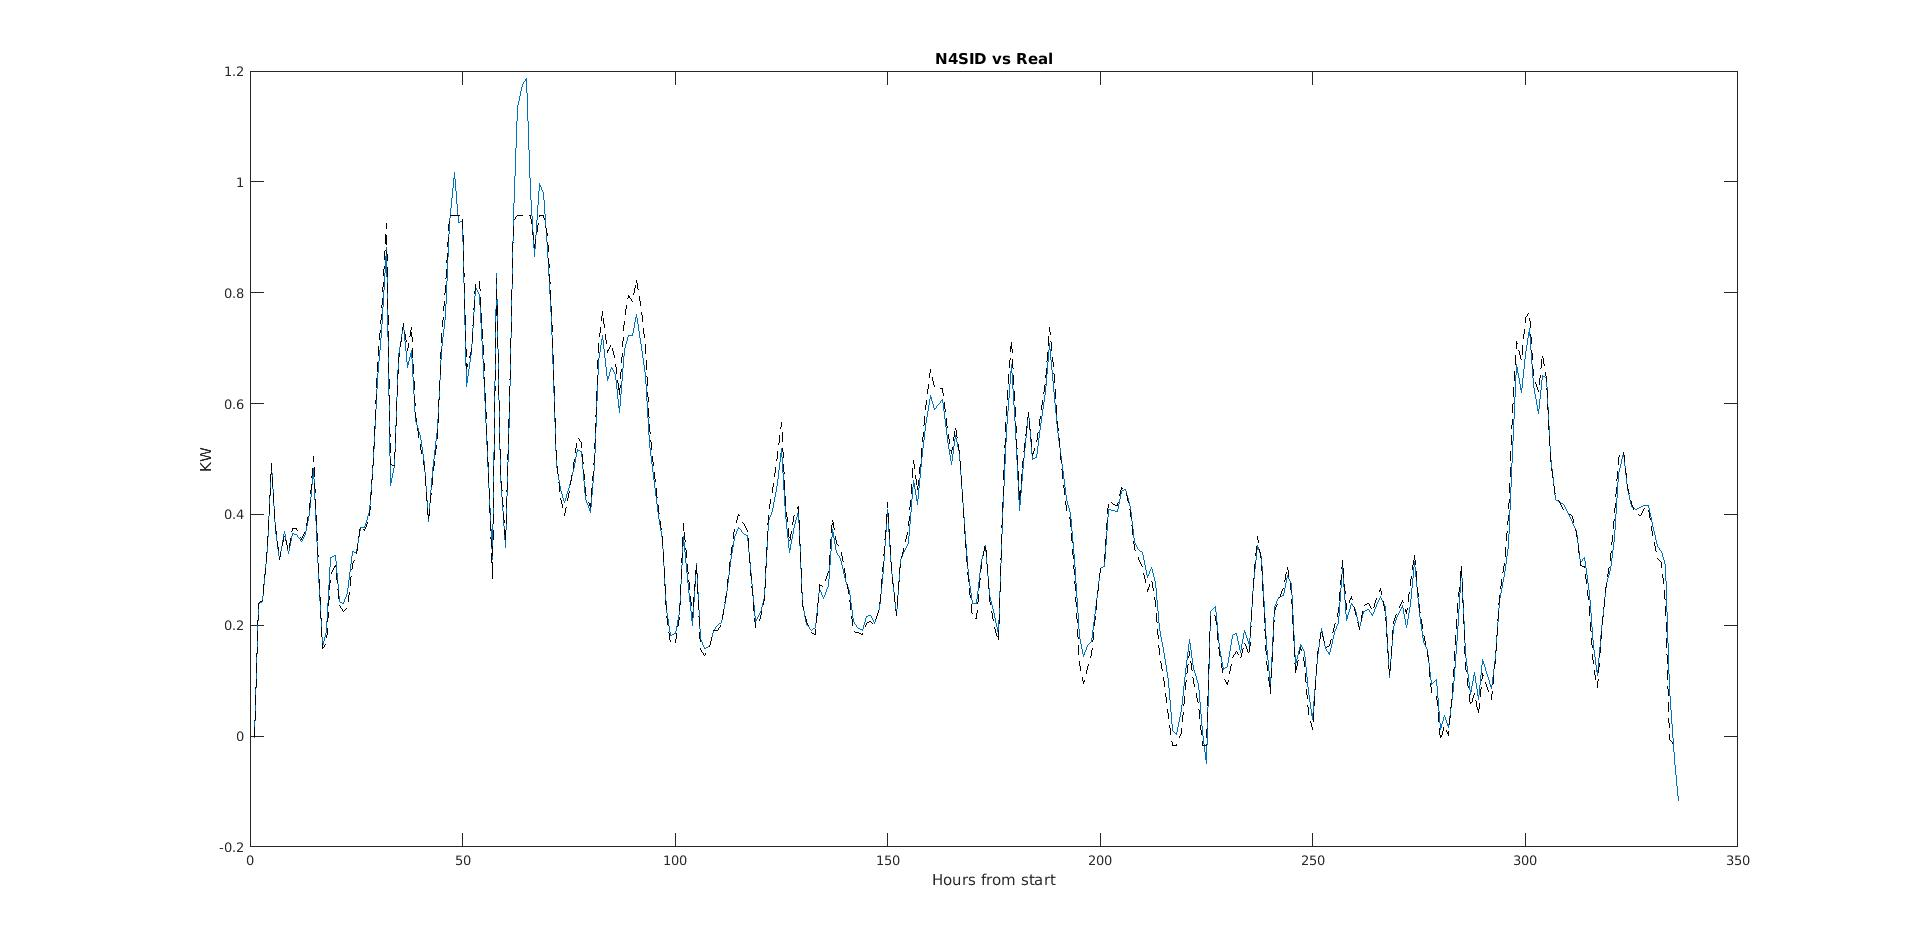
\includegraphics[width=\textwidth]{n4sid_eolica.jpg}
    \caption{N4SID Prediction accurancy}
\end{figure}

\begin{figure}[h]
    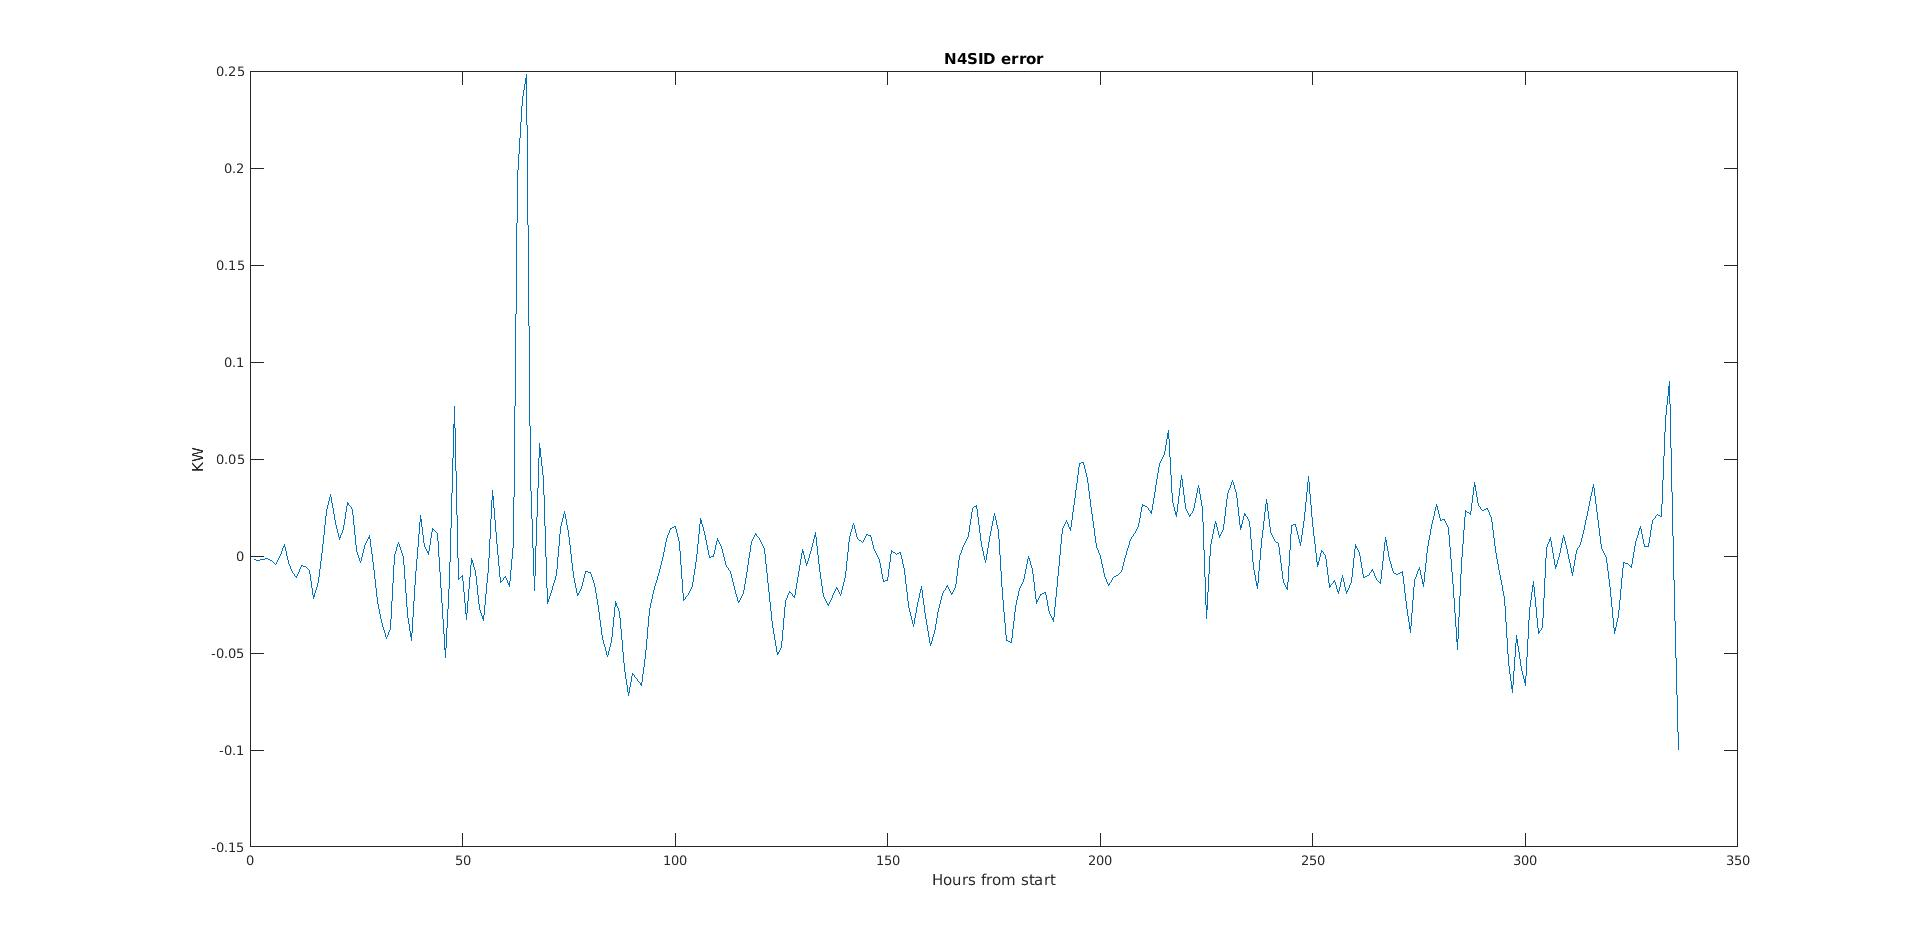
\includegraphics[width=\textwidth]{n4sid_eolica_error.jpg}
    \caption{N4SID Prediction error}
\end{figure}


\subsubsection{Eólica: ARIMA/ARMA} % (fold)
\label{ssub:eólica_arima_arma}

\begin{figure}[h]
    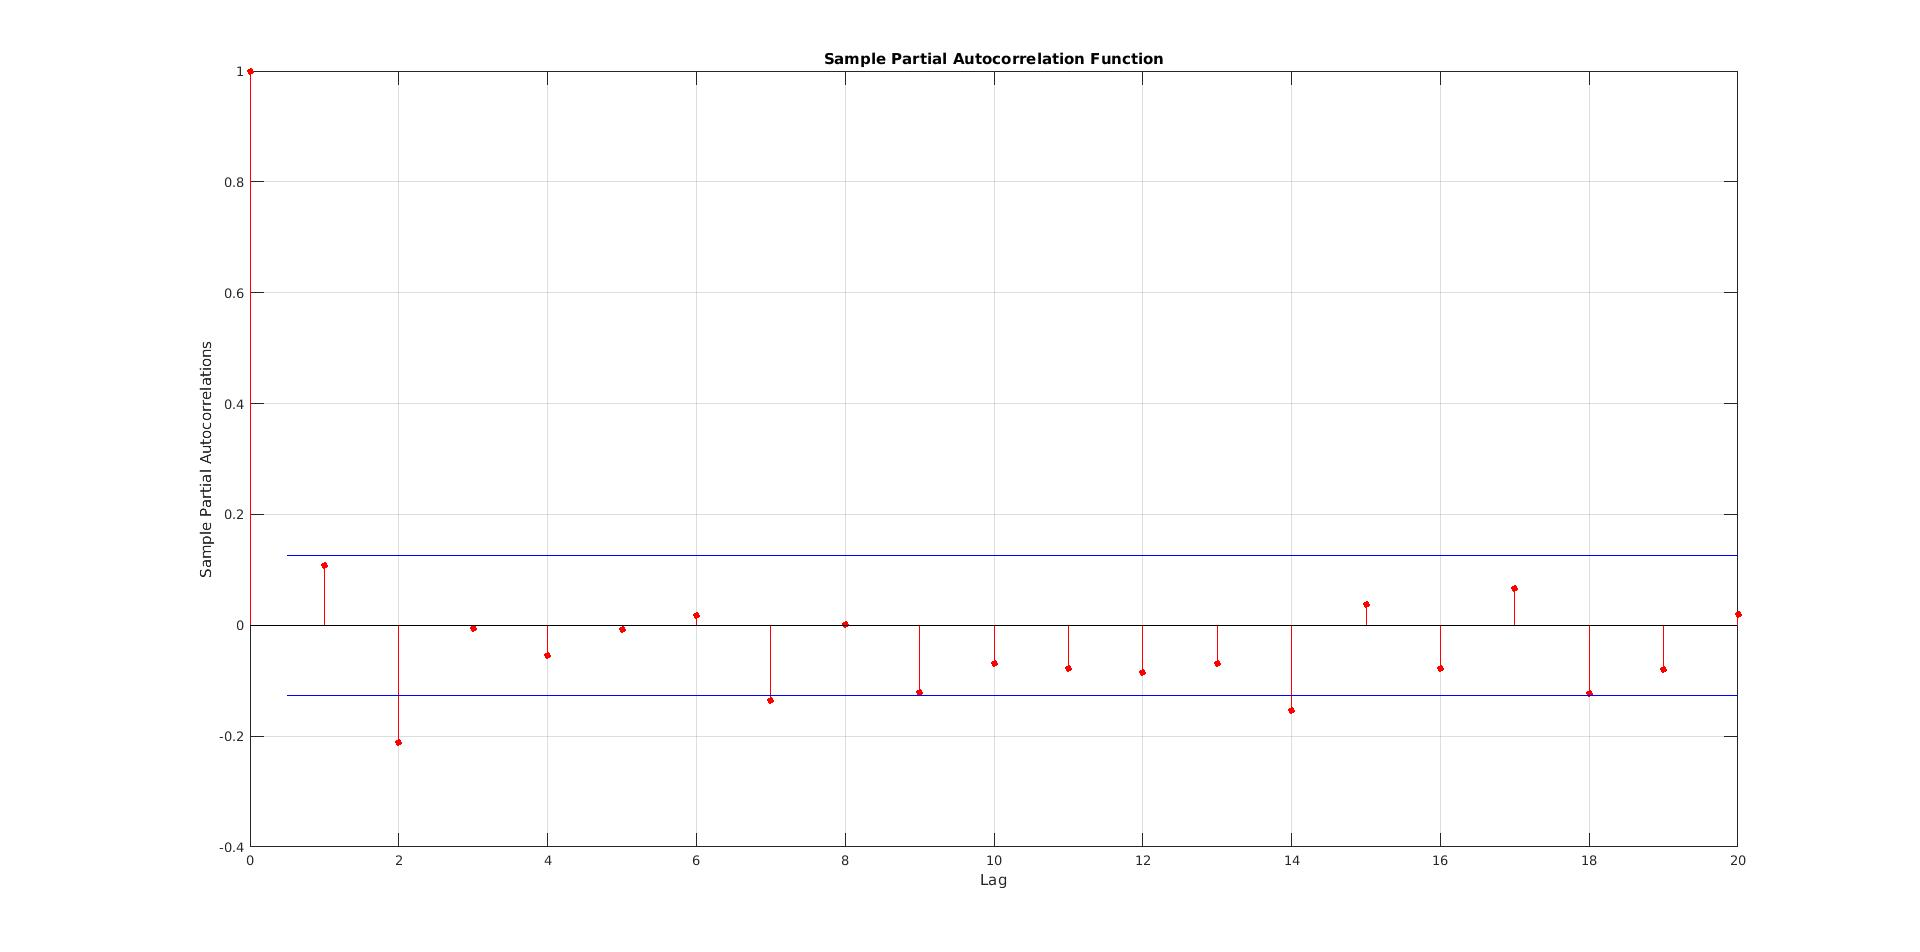
\includegraphics[width=\textwidth]{arma_partial_autocorrelation.jpg}
    \caption{N4SID Prediction accurancy}
\end{figure}
\begin{figure}[h]
    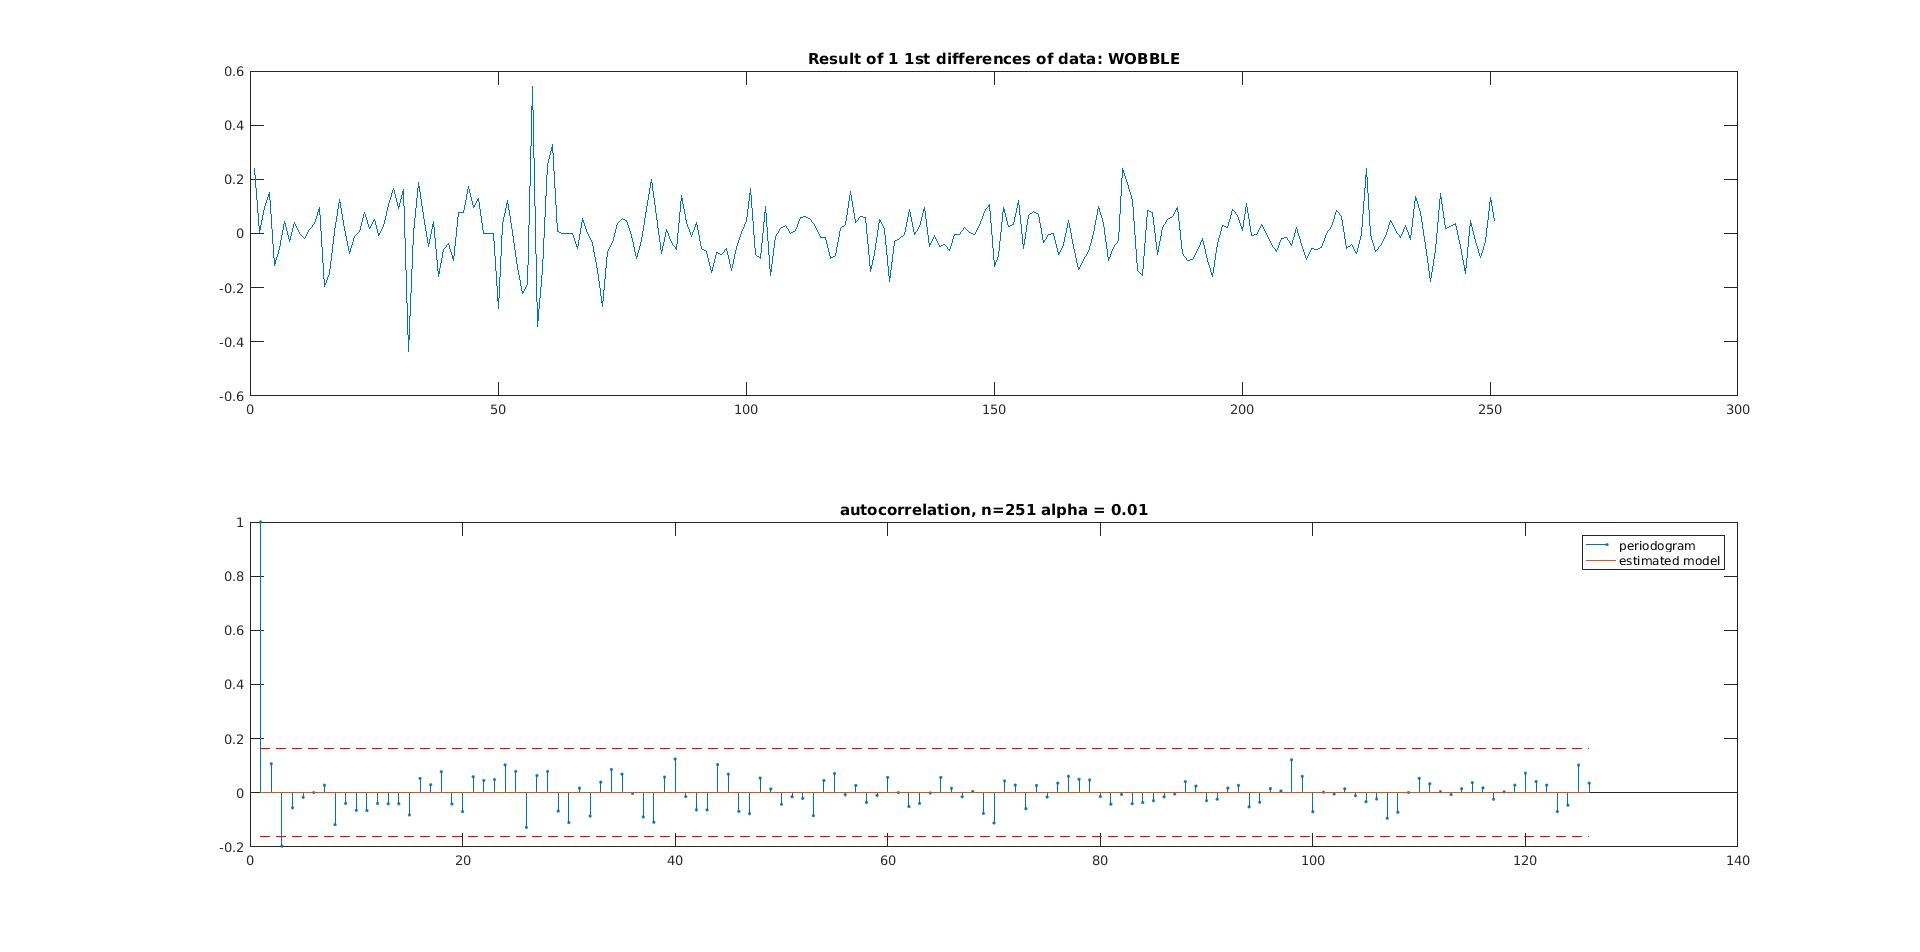
\includegraphics[width=\textwidth]{arma_differenciation.jpg}
    \caption{N4SID Prediction accurancy}
\end{figure}
\begin{figure}[h]
    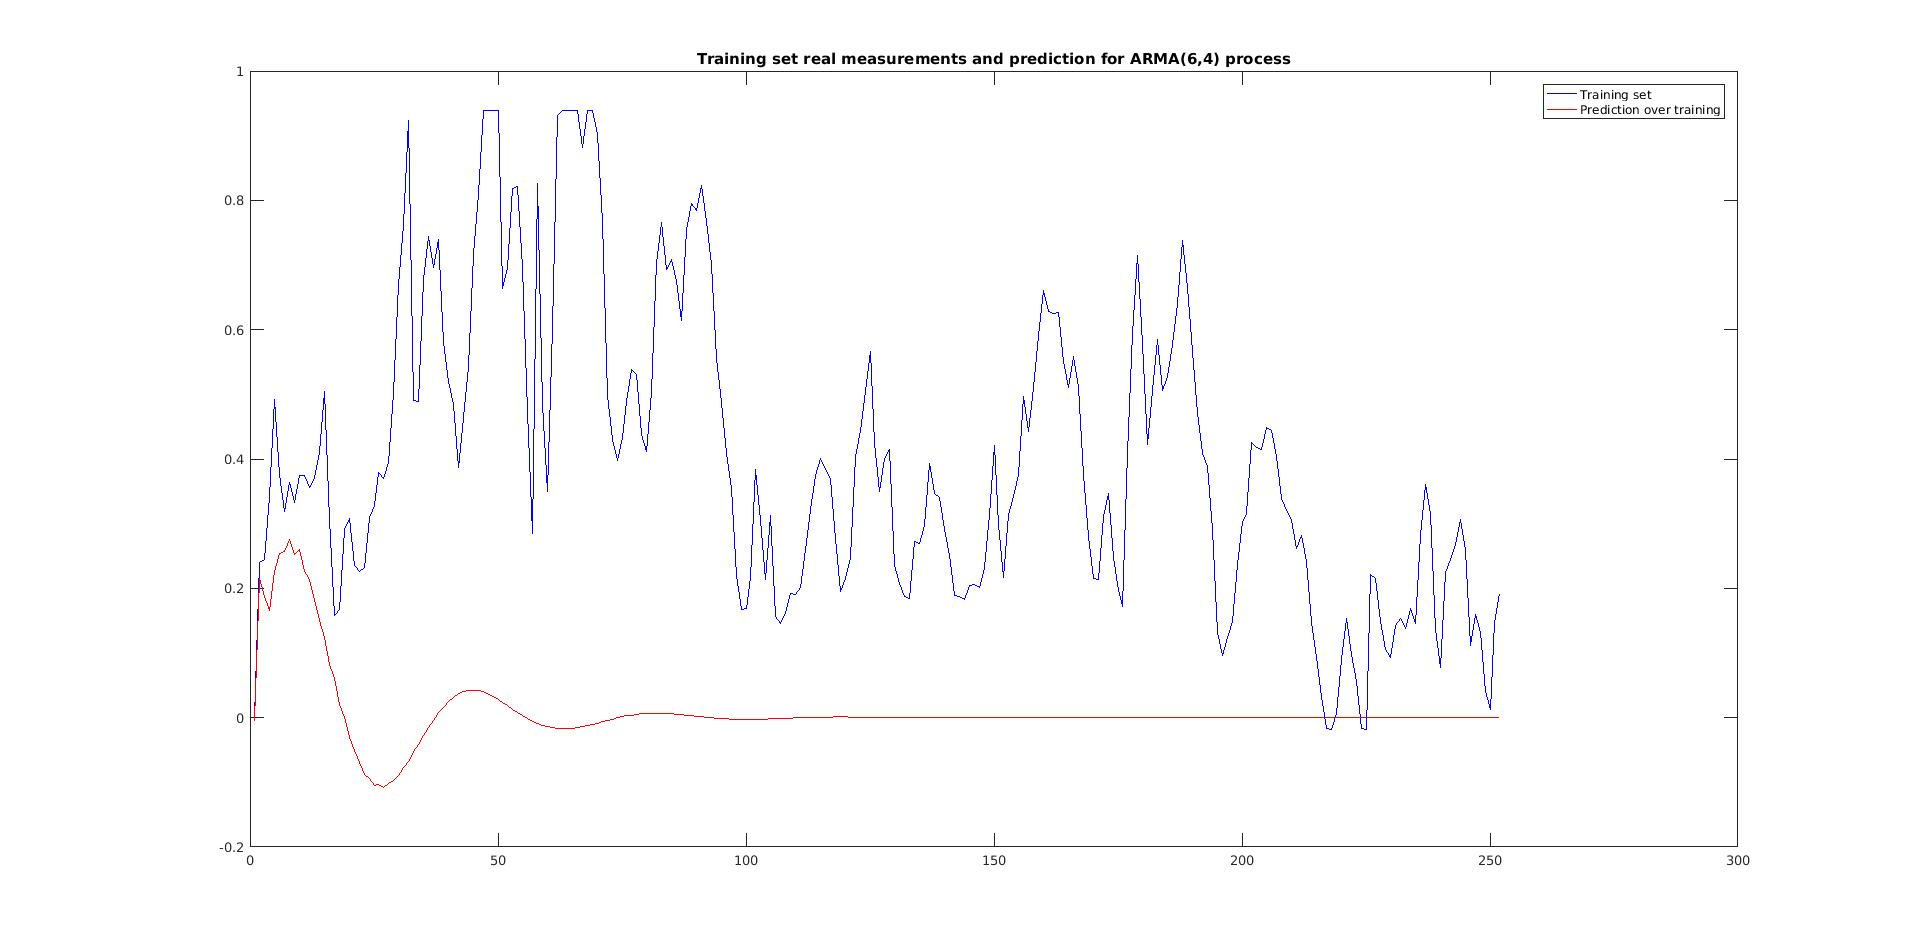
\includegraphics[width=\textwidth]{arma_train_and_predictionOverTrain.jpg}
    \caption{N4SID Prediction accurancy}
\end{figure}
\begin{figure}[h]
    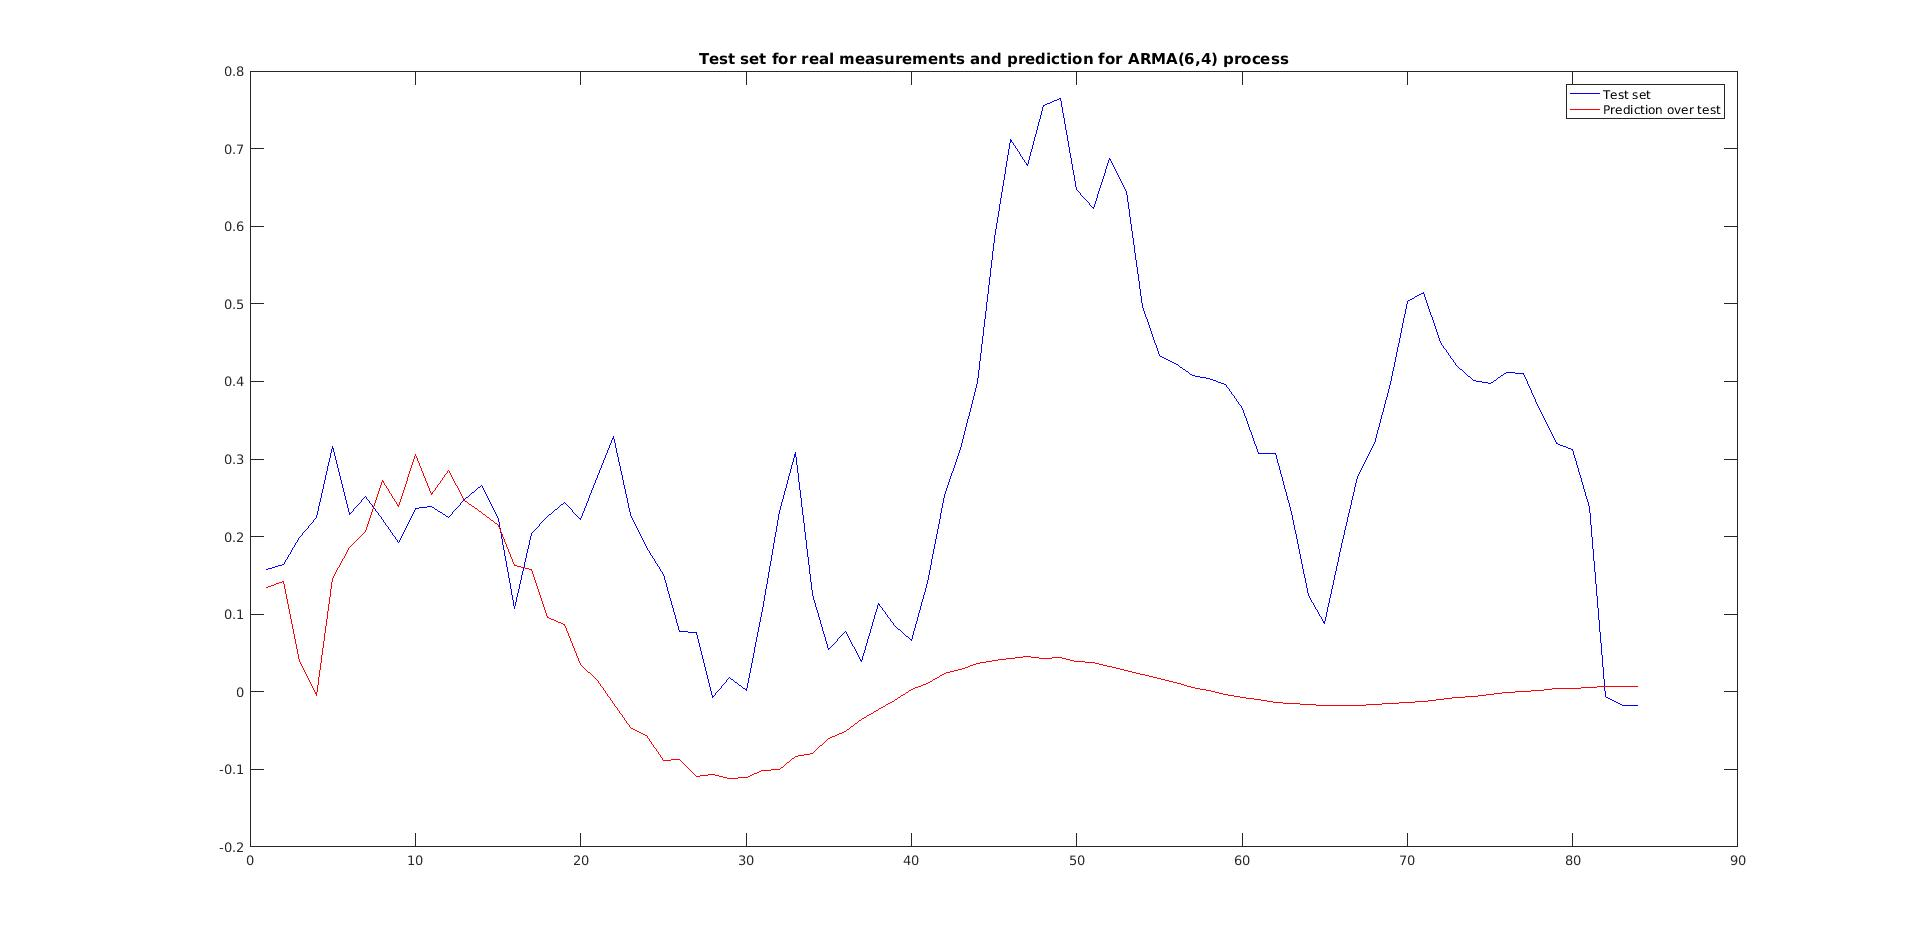
\includegraphics[width=\textwidth]{arma_test_and_predictionOverTest.jpg}
    \caption{N4SID Prediction accurancy}
\end{figure}